%===============================================================================
% LaTeX sjabloon voor de bachelorproef toegepaste informatica aan HOGENT
% Meer info op https://github.com/HoGentTIN/bachproef-latex-sjabloon
%===============================================================================

\documentclass{bachproef-tin}

\usepackage{hogent-thesis-titlepage} % Titelpagina conform aan HOGENT huisstijl

%%---------- Documenteigenschappen ---------------------------------------------

% De titel van het rapport/bachelorproef
\title{ICT binnen educatie in Peru, een stand van zaken en suggesties tot optimalisatie}

\author{Lucas Vermeulen}

% De naam van je promotor (lector van de opleiding)
\promotor{Joeri Van Herreweghe}

% De naam van je co-promotor. Als je promotor ook je opdrachtgever is en je
% dus ook inhoudelijk begeleidt (en enkel dan!), mag je dit leeg laten.
\copromotor{Ellen Bosch}

% Indien je bachelorproef in opdracht van/in samenwerking met een bedrijf of
% externe organisatie geschreven is, geef je hier de naam. Zoniet laat je dit
% zoals het is.
\instelling{---}

% Academiejaar
\academiejaar{2019-2020}

% Examenperiode
%  - 1e semester = 1e examenperiode => 1
%  - 2e semester = 2e examenperiode => 2
%  - tweede zit  = 3e examenperiode => 3
\examenperiode{2}

%===============================================================================
% Inhoud document
%===============================================================================

\begin{document}

%---------- Taalselectie -------------------------------------------------------
% Als je je bachelorproef in het Engels schrijft, haal dan onderstaande regel
% uit commentaar. Let op: de tekst op de voorkaft blijft in het Nederlands, en
% dat is ook de bedoeling!

%\selectlanguage{english}

%---------- Titelblad ----------------------------------------------------------
\inserttitlepage

%---------- Samenvatting, voorwoord --------------------------------------------
\usechapterimagefalse
%%=============================================================================
%% Voorwoord
%%=============================================================================

\chapter*{Woord vooraf}
\label{ch:voorwoord}

%% TODO:
%% Het voorwoord is het enige deel van de bachelorproef waar je vanuit je
%% eigen standpunt (``ik-vorm'') mag schrijven. Je kan hier bv. motiveren
%% waarom jij het onderwerp wil bespreken.
%% Vergeet ook niet te bedanken wie je geholpen/gesteund/... heeft

Op 2 mei begon mijn stage in Cusco, Peru. Ik liep stage bij Añañau, een organisatie die zich inzet om kinderen en jongeren een betere toekomst te geven. Añañau is voornamelijk een onderwijs project. Het project werd opgericht door Ellen Bosch en Sadith Paez Montesinos. Ik koos voor deze stage omdat ik denk dat ik zelf veel kan bijleren over hoe men de dingen doet in een land zoals Peru. Ook werken met de kinderen sprak me echt aan, in combinatie met mijn studie en passie: informatica. Als eerst informatica student die stage deed bij Añañau kreeg ik veel algemene IT vragen waarvoor ik een oplossing zocht. Daarnaast schreef ik er twee applicaties voor het project: een bibliotheek-applicatie en een applicatie om nieuwe stagiairs of vrijwilligers de kans te geven om zich te registreren. 

Ik wou graag mijn bachelorproef onderzoek doen rond iets waarmee ik in aanraking kwam tijdens mijn stage. Ik wist van een eerdere uitwisseling, na mijn middelbaar onderwijs in Ecuador (een buurland in het noorden van Peru), hoever het onderwijs daar stond en hoe ze daar omgingen met informatica. Ik wist dus waaraan ik me kon verwachten. Het was bijgevolg ideaal om het informatica-aspect uit mijn studies te combineren met het onderwijs-aspect van het project. 

Tijdens de stage die ik liep in Peru verspreidde het covid-19 virus zich over de wereld. Ook Peru werd getroffen. Ondanks het feit dat de meeste besmettingen in Lima te situeren waren en Cusco relatief gespaard bleef, was het beter om terug te keren naar België en mijn stage vanop afstand verder te zetten. Ook dit bachelorproef-onderzoek moest volledig vanop afstand gebeuren door de opgelegde maatregelen, wat uiteraard erg jammer was.

Tijdens het schrijven werd ik door een aantal mensen geholpen. Eerst en vooral wens ik mijn co-promotor Mevr. Ellen Bosch hartelijk te bedanken. Zei gaf me - voor ik startte met mijn onderzoek - goede raad en een duidelijke richting mee, waardoor ik veel beter wist wat me te doen stond. Ook op tussentijds basis evalueerde ze samen met Dhr. Joeri Van Herreweghe, mijn promoter, wat ik had geschreven, wat ik heel erg apprecieerde. Bedankt! Daarnaast wens ik Mvr. Sadith Paez Montesinos te bedanken. Ze hielp me aan contactpersonen van wie een interview kon afnemen en bezorgde me informatie over mijn onderzoeksdomein. Ook een speciale bedanking aan Dhr. Erick Paez Montesinos en Mvr. Carmen Rosa Diaz Fonseca die ik kon interviewen tijdens het onderzoek, en aan mijn ouders om mij te steun door dik en dun.

Ik wens u veel leesplezier toe,

Lucas Vermeulen

29 mei, Gent
%%=============================================================================
%% Samenvatting
%%=============================================================================

% TODO: De "abstract" of samenvatting is een kernachtige (~ 1 blz. voor een
% thesis) synthese van het document.
%
% Deze aspecten moeten zeker aan bod komen:
% - Context: waarom is dit werk belangrijk?
% - Nood: waarom moest dit onderzocht worden?
% - Taak: wat heb je precies gedaan?
% - Object: wat staat in dit document geschreven?
% - Resultaat: wat was het resultaat?
% - Conclusie: wat is/zijn de belangrijkste conclusie(s)?
% - Perspectief: blijven er nog vragen open die in de toekomst nog kunnen
%    onderzocht worden? Wat is een mogelijk vervolg voor jouw onderzoek?
%
% LET OP! Een samenvatting is GEEN voorwoord!

%%---------- Nederlandse samenvatting -----------------------------------------
%
% TODO: Als je je bachelorproef in het Engels schrijft, moet je eerst een
% Nederlandse samenvatting invoegen. Haal daarvoor onderstaande code uit
% commentaar.
% Wie zijn bachelorproef in het Nederlands schrijft, kan dit negeren, de inhoud
% wordt niet in het document ingevoegd.

\IfLanguageName{english}{%
\selectlanguage{dutch}
\chapter*{Samenvatting}
\lipsum[1-4]
\selectlanguage{english}
}{}

%%---------- Samenvatting -----------------------------------------------------
% De samenvatting in de hoofdtaal van het document

\chapter*{\IfLanguageName{dutch}{Samenvatting}{Abstract}}

%\lipsum[1-4]


%---------- Inhoudstafel -------------------------------------------------------
\pagestyle{empty} % Geen hoofding
\tableofcontents  % Voeg de inhoudstafel toe
\cleardoublepage  % Zorg dat volgende hoofstuk op een oneven pagina begint
\pagestyle{fancy} % Zet hoofding opnieuw aan

%---------- Lijst figuren, afkortingen, ... ------------------------------------

% Indien gewenst kan je hier een lijst van figuren/tabellen opgeven. Geef in
% dat geval je figuren/tabellen altijd een korte beschrijving:
%
%  \caption[korte beschrijving]{uitgebreide beschrijving}
%
% De korte beschrijving wordt gebruikt voor deze lijst, de uitgebreide staat bij
% de figuur of tabel zelf.

\listoffigures
%\listoftables

% Als je een lijst van afkortingen of termen wil toevoegen, dan hoort die
% hier thuis. Gebruik bijvoorbeeld de ``glossaries'' package.
% https://www.overleaf.com/learn/latex/Glossaries

%---------- Kern ---------------------------------------------------------------

% De eerste hoofdstukken van een bachelorproef zijn meestal een inleiding op
% het onderwerp, literatuurstudie en verantwoording methodologie.
% Aarzel niet om een meer beschrijvende titel aan deze hoofstukken te geven of
% om bijvoorbeeld de inleiding en/of stand van zaken over meerdere hoofdstukken
% te verspreiden!

\chapter{Inleiding}
\label{ch:inleiding}

Onderwijs is een belangrijke factor in de groei en ontwikkeling van een land. Elk onderwijssysteem van elk land heeft andere kenmerken, noden en kwaliteiten. Informatica is niet meer uit onze maatschappij weg te denken. Op scholen moet men alle trends kunnen volgen, wat niet altijd even eenvoudig blijkt. Dit onderzoek richt zich op informatica in educatie in Peru. Het bekijkt hoe het staat met informatica in het onderwijs, en er worden suggesties tot optimalisatie gedaan.

Peru is een Zuid-Amerikaans ontwikkelingsland. Er heerst zowel in de grote steden als in het binnenland veel armoede. Vooral in het staatsonderwijs zijn de gevolgen daarvan duidelijk. Het onderwijs in Peru bestaat uit publieke scholen en private scholen. Publieke scholen of staatsscholen zijn toegankelijk voor iedereen. Voor private scholen moeten kinderen toegelaten worden en meestal maandelijks betalen. In het algemeen geldt er dat de kinderen van arme gezinnen naar staatsscholen gaan en de kinderen van rijkere gezinnen naar private scholen. Omdat staatsscholen voor iedereen toegankelijk zijn is dit onderzoek volledig gebaseerd op het staatsonderwijs. Er zal onderzoek gedaan worden naar de huidige stand van zaken van ICT binnen het staatsonderwijs in Peru en er zal naar optimalisaties gezocht worden. Dit zal gebeuren op basis van interviews waarna er conclusies getrokken zullen worden.

%De inleiding moet de lezer net genoeg informatie verschaffen om het onderwerp te begrijpen en in te zien waarom de onderzoeksvraag de moeite waard is om te onderzoeken. In de inleiding ga je literatuurverwijzingen beperken, zodat de tekst vlot leesbaar blijft. Je kan de inleiding verder onderverdelen in secties als dit de tekst verduidelijkt. Zaken die aan bod kunnen komen in de inleiding~\autocite{Pollefliet2011}:

%\begin{itemize}
%  \item context, achtergrond
%  \item afbakenen van het onderwerp
%  \item verantwoording van het onderwerp, methodologie
%  \item probleemstelling
%  \item onderzoeksdoelstelling
%  \item onderzoeksvraag
%  \item \ldots
%\end{itemize}

\section{Probleemstelling}
\label{sec:probleemstelling}
Veel ontwikkelingslanden hebben te maken met een zogenaamde "digital gap". Ze hebben een achterstand op vlak van informatica tegenover beter ontwikkelde landen. Informatica is erg belangrijk in de ontwikkeling van een land. Onderwijs kan aan de basis liggen om dit probleem te verhelpen. Door kinderen op te leiden en ze te voorzien van know-how kan het land de digital gap proberen te dichten. Zowel de overheid als leerlingen en scholen hebben baat bij een goede implementatie van informatica in het onderwijs. 

%Uit je probleemstelling moet duidelijk zijn dat je onderzoek een meerwaarde heeft voor een concrete doelgroep. De doelgroep moet goed gedefinieerd en afgelijnd zijn. Doelgroepen als ``bedrijven,'' ``KMO's,'' systeembeheerders, enz.~zijn nog te vaag. Als je een lijstje kan maken van de personen/organisaties die een meerwaarde zullen vinden in deze bachelorproef (dit is eigenlijk je steekproefkader), dan is dat een indicatie dat de doelgroep goed gedefinieerd is. Dit kan een enkel bedrijf zijn of zelfs één persoon (je co-promotor/opdrachtgever).

\section{Onderzoeksvragen}
\label{sec:onderzoeksvraag}

%Wees zo concreet mogelijk bij het formuleren van je onderzoeksvraag. Een onderzoeksvraag is trouwens iets waar nog niemand op dit moment een antwoord heeft (voor zover je kan nagaan). Het opzoeken van bestaande informatie (bv. ``welke tools bestaan er voor deze toepassing?'') is dus geen onderzoeksvraag. Je kan de onderzoeksvraag verder specifiëren in deelvragen. Bv.~als je onderzoek gaat over performantiemetingen, dan 

$Onderzoeksvraag$ 1: Wat is de huidige stand van zaken op vlak van ICT binnen het onderwijs in Peru, en hoe is het land hiertoe gekomen?

$Onderzoeksvraag$ 2: Hoe kunnen deze knelpunten weggewerkt worden in de toekomst?

\section{Onderzoeksdoelstelling}
\label{sec:onderzoeksdoelstelling}

%Wat is het beoogde resultaat van je bachelorproef? Wat zijn de criteria voor succes? Beschrijf die zo concreet mogelijk. Gaat het bv. om een proof-of-concept, een prototype, een verslag met aanbevelingen, een vergelijkende studie, enz.

De doelstelling van dit onderzoek is het erkennen en correct formuleren van de pijnpunten van ICT binnen het onderwijs in Peru. Er worden ook suggesties gedaan om de knelpunten te optimaliseren.

\section{Opzet van deze bachelorproef}
\label{sec:opzet-bachelorproef}

% Het is gebruikelijk aan het einde van de inleiding een overzicht te
% geven van de opbouw van de rest van de tekst. Deze sectie bevat al een aanzet
% die je kan aanvullen/aanpassen in functie van je eigen tekst.

Deze bachelorproef is als volgt opgebouwd:

In Hoofdstuk~\ref{ch:stand-van-zaken} wordt een overzicht gegeven van de stand van zaken binnen het onderzoeksdomein, op basis van een literatuurstudie.

In Hoofdstuk~\ref{ch:methodologie} wordt de methodologie toegelicht en worden de gebruikte onderzoekstechnieken besproken om een antwoord te kunnen formuleren op de onderzoeksvragen.

In Hoofdstuk~\ref{ch:interviewSadith} wordt een interview met Sadith Paez Montesinos, één van de mede-oprichtsters van Añañau besproken.

In Hoofdstuk~\ref{ch:interviewRosa} wordt een interview met Rosa Diaz Fonseca, een ex-medewerker van het Peruviaanse ministerie van onderwijs en schooldirectrice besproken.

In Hoofdstuk~\ref{ch:interviewErick} wordt een interview met Erick Paez Montesinos, een ex-medewerker van het Peruviaanse ministerie van onderwijs en leerkracht besproken.

In Hoofdstuk~\ref{ch:conclusie}, tenslotte, worden conclusies getrokken en wordt een antwoord geformuleerd op de verschillende onderzoeksvragen. Daarbij wordt ook een aanzet gegeven voor toekomstig onderzoek binnen dit domein.
\chapter{\IfLanguageName{dutch}{Stand van zaken}{State of the art}}
\label{ch:stand-van-zaken}

% Tip: Begin elk hoofdstuk met een paragraaf inleiding die beschrijft hoe
% dit hoofdstuk past binnen het geheel van de bachelorproef. Geef in het
% bijzonder aan wat de link is met het vorige en volgende hoofdstuk.

% Pas na deze inleidende paragraaf komt de eerste sectiehoofding.

%Dit hoofdstuk bevat je literatuurstudie. De inhoud gaat verder op de inleiding, maar zal het onderwerp van de bachelorproef *diepgaand* uitspitten. De bedoeling is dat de lezer na lezing van dit hoofdstuk helemaal op de hoogte is van de huidige stand van zaken (state-of-the-art) in het onderzoeksdomein. Iemand die niet vertrouwd is met het onderwerp, weet nu voldoende om de rest van het verhaal te kunnen volgen, zonder dat die er nog andere informatie moet over opzoeken \autocite{Pollefliet2011}.

%Je verwijst bij elke bewering die je doet, vakterm die je introduceert, enz. naar je bronnen. In \LaTeX{} kan dat met het commando \texttt{$\backslash${textcite\{\}}} of \texttt{$\backslash${autocite\{\}}}. Als argument van het commando geef je de ``sleutel'' van een ``record'' in een bibliografische databank in het Bib\LaTeX{}-formaat (een tekstbestand). Als je expliciet naar de auteur verwijst in de zin, gebruik je \texttt{$\backslash${}textcite\{\}}.
%Soms wil je de auteur niet expliciet vernoemen, dan gebruik je \texttt{$\backslash${}autocite\{\}}. In de volgende paragraaf een voorbeeld van elk.

%\textcite{Knuth1998} schreef een van de standaardwerken over sorteer- en zoekalgoritmen. Experten zijn het erover eens dat cloud computing een interessante opportuniteit vormen, zowel voor gebruikers als voor dienstverleners op vlak van informatietechnologie~\autocite{Creeger2009}.

%-----------------------------------
% BESPREKING ELLEN

%waar staat peru in ontwikkeling op vlak van ict
%digital gap
%duurzame ontwikkelingsdoelen agenda 2030 vn = SDG 
%17 logo's
%SDG --> ICT
%milenium doelstellingen 2015
%
%peru in het algemeen
%als ontwikkelingsland --> vn/SDG
%hegt onderwijs in peru
%ict 
%digital gap 
%projecten in het verleden/organisaties ict hulp?
%
%
%vlirous - project beurs - peru project -computers recycleren

\section{Peru: een bloemlezing}
In dit hoofdstuk worden verschillende kenmerken van het land Peru besproken. 
\subsection{Geografisch}
Peru ligt aan de westkust van zuid-Amerika. Het grenst in het noorden aan Colombia en Ecuador, in het oosten aan Bolivia en Brazilië en in het zuiden aan Chili. Aan de westkust van het land ligt de Grote Oceaan. Lima is de hoofdstad van het land, en telt ruim 10 miljoen inwoners. Qua oppervlakte is Peru 42 keer zo groot als België, het meet 1.285.216 km\textsuperscript{2}. 

\subsubsection{Landschap}
In Peru kunnen er 3 verschillende soorten landschap gevonden worden: het kustgebied, de bergen en de jungle. De kust van Peru bestaat uit woestijn die tussen de zee en de bergen ligt. Het Andes gebergte is het belangrijkste gebergte van het land en daarachter ligt de jungle. Die kan opgesplitst worden in 2 verschillende stukken: er is het hoge regenwoud, dat op 700 meter hoogte ligt en de amazone-jungle waar de Amazone rivier door stroomt. \autocite{ToPeru2020}

\subsection{Demografisch}
Peru heeft op dit moment 32 miljoen inwoners \autocite{Overheid2020}. Officieel worden er drie talen gesproken: Spaans, Quechua en Aymara. 
Met ongeveer 3,3 miljoen sprekers wordt Quechua beschouwd als de meest gesproken moedertaal in Peru. Naast Peru wordt Quechua ook gesproken in 6 andere Zuid-Amerikaanse landen: Ecuador, Colombia, Bolivia, Argentinië, Chili en Brazilië. \autocite{Cultura2020}
Aymara is een taal die tot de familie van Aru behoort. Ze wordt gesproken door ongeveer 450.000 mensen. \autocite{CulturaPeru2020} Ze wordt ook gesproken in Bolivia en Noord-Argentinië en Chili. In de Amazone worden bovendien 70 verschillende onofficiële, lokale talen gesproken. \autocite{dosmanosperu}

\subsection{Cultuur en Economie}
De nationale feestdag van Peru valt op 28 Juli. In Peru worden deze dagen de Fiestas Patrias genoemd. \autocite{dosmanosperu2018} Verder wordt er in Peru betaald met de Peruviaanse sol. Op dit moment is 1 Euro ongeveer gelijk aan 3,82 Peruviaanse sol.

\section{Peru als ontwikkelingsland}
\subsection{Wat is een ontwikkelingsland?}
Volgens het boek Grondlijnen van internationaal recht, \autocite{MarcJ.Bossuyt2005}, bestaat er geen algemene definitie voor een ontwikkelingsland. Dat komt omdat de verschillende internationale instellingen, die zich bezig houden met het quoteren van landen, verschillende criteria gebruiken. Daarnaast is het soms niet duidelijk wat er met ontwikkeling bedoeld wordt.
De status van een ontwikkelingsland is niet permanent, een land kan zich verder ontwikkelen.

\subsection{Indeling van ontwikkelingslanden}
De indeling van ontwikkelingslanden kan op twee manieren gedaan worden. De eerste is door middel van abstracte criteria, de tweede door middel van lijsten. Een abstract criterium wordt op alle landen gelijk toegepast. Alle landen die onder een vooraf bepaalde grens vallen zijn dan ontwikkelingslanden, de anderen zijn dan ontwikkelde landen. Een lijst is een volledige opsomming, van items die gebaseerd zijn op onbetrouwbare of onbestaande statistieken, waaraan een land moet voldoen. \autocite{MarcJ.Bossuyt2005},

In het "World Economic Situation and Prospects 2019" rapport \autocite{unitednations2019} deelt de Verenigde Naties alle landen in drie grote groepen op. Volgens de VN zijn er 43 ontwikkelde landen, 17 landen die de overgang maken tussen onderontwikkeld en ontwikkeld land en maar liefst 127 landen die als onderontwikkeld worden beoordeeld. België behoort (uiteraard) tot de ontwikkelde landen, Peru tot de onderontwikkelde landen. \autocite{unitednations2019}

De VN stelde dat deze verdeling niet perfect is. Ze konden niet alle ontwikkelingslanden over dezelfde kam scheren, omdat er landen waren die soms meer aandacht verdienden dan anderen op vlak van internationale ontwikkelingssamenwerking. De VN stelde naast ontwikkelde landen in overgang en onderontwikkelde landen, nog drie andere groepen op, om de onderontwikkelde landen in op de delen: 

\begin{itemize}
\item De minst ontwikkelde landen, (least developed country's of LDC);
\item De ontwikkelingslanden zonder zeekust, (landlocked developing countries of LLDC);
\item de kleine eilandstaten in ontwikkeling, (Small island developing states of SIDS).
\end{itemize}
\autocite{MarcJ.Bossuyt2005},

Een land kan tot meerdere categorieën behoren. De lijsten worden elke 3 jaar door ECOSOC (United Nations Department of Economic and Social Affairs) in de verschillende groepen opgedeeld. \autocite{ecosoc2018} In 2018 deed ECOSOC dat, en waren er 47 LDC's, 31 LLDC's en 48 SIDS. Peru behoort niet tot een van deze groepen. \autocite{MarcJ.Bossuyt2005},

\subsection{Human development index}
De human development index (HDI) geeft landen een score. Dit gebeurt door elk land te quoteren op vlak van verschillende dimensies. De quoteringsvlakken die in acht worden genomen zijn de onderwijsdimensie, de gezondheidsdimensie en de levensstandaard dimensie.

De gezondheidsdimensie wordt beoordeeld aan de hand van de levensverwachting bij de geboorte. De onderwijsdimensie wordt gemeten aan de hand van het aantal verwacht aantal schooljaren voor volwassenen van 25 jaar en verwachte schooljaren voor schoolgaande kinderen. Tot slot wordt de levensstandaard dimensie gemeten aan de hand van het bruto nationaal inkomen per inwoner. De HDI werd gemaakt om te benadrukken dat mensen en hun capaciteiten de ultieme criteria moeten zijn voor het beoordelen van de ontwikkeling van een land, en niet alleen economische groei. \autocite{UNDP2019}

Met de scores die resulteren uit de berekening, kan een rangschikking gevormd worden. Die rangschikking kan dan duiden op welk land beter ontwikkelt tegenover andere landen. 

Sinds 1990 heeft het Ontwikkelingsprogramma van de Verenigde Naties (UNDP) in zijn jaarlijkse Human Development Reports, de Human development index voor elk land gepubliceerd. \autocite{AmbujD.Sagar1997}. Deze index is een belangrijk alternatief voor de traditionele eendimensionale maatstaf voor ontwikkeling (BBP). 

België stond in 2019 op de 17de plaats, Peru op de 82ste. Bovenaan de lijst triomfeert Noorwegen. \autocite{UNDP2019a} 

\subsubsection{Kritiek op de HDI}
Er kwam kritiek op de indicator aangezien hij enkel sociale factoren in rekening brengt. Sinds 2010 gebruikt de VN een aangepaste versie van de indicator: de index van duurzame menselijke ontwikkeling (HSDI) die ook de koolstofemissies per capita in rekening brengt. \autocite{Economie2018}

\subsection{Armoede en ongelijkheid in Peru}
Armoede en ongelijkheid zijn twee begrippen die vaak in één adem met elkaar worden genoemd. Ze hebben ook veel met elkaar te maken, maar staan los van elkaar. Je kunt in je ééntje arm zijn, maar je kunt niet in je ééntje ongelijk zijn. Kort gezegd betekent ‘armoede’ dat je ergens een tekort aan hebt. Bij ongelijkheid gaat het erom dat (minimaal) 2 mensen niet dezelfde kansen krijgen (of dezelfde toegang hebben tot eenzelfde middel). \autocite{Novib2020}

\subsubsection{Armoede in Peru}
Volgens \autocite{OurWorldInData2016} leefde 17.90\% van de bevolking in 1997 in extreme armoede. In 2014 was dat 3.70\%. Onder extreme armoede verstaat de Wereld Bank mensen die minder dan 1,90 dollar per dag kunnen uitgeven om te leven. De daling van 17.90\% naar 3.70\% lijkt heel groot, maar nog steeds leven er ongeveer 1,125 miljoen mensen in armoede. Deze grens ligt heel erg laag. Het is dus ook interessant om die grens te verhogen, en te kijken hoeveel mensen er met 3,10 dollar per dag moeten leven. In 1997 was dat 32,07\% van de Peruviaanse bevolking en in 2016  9.01\%.

\subsection{Ongelijkheid in Peru}
De economische ongelijkheid ontstaat vooral doordat de vermogens in bepaalde landen ongelijk verdeeld zijn. De oorzaak hiervan is dat kapitaal zich ofwel in privéhanden bevindt of in handen van de overheid, die ze niet goed beheert. \autocite{Zucman2018}

Ongelijkheid kan gemeten worden door de GINI-index. De GINI-index is een statistische verdelingsmaatregel, die in 1912 ontwikkeld werd door de Italiaanse statisticus Corrado Gini. Het wordt vaak gebruikt als maatstaf voor economische ongelijkheid, om de inkomensverdeling te meten. Het geeft landen, een score tussen 0 en 1, waarbij 0 voor perfecte gelijkheid staat en 1 voor perfecte ongelijkheid.  \autocite{Chappelow2020}

De Gini-index voor belgie was in 2017 0.274, voor Peru was die in 2018 0.428. \autocite{Bank2018}

%ELLEN: In dit hoofdstuk en zijn onderverdelingen geef je heel goed weer waar Peru op wereldvlak staat als ontwikkelingsland volgens de verschillende indelingen. Na dit hoofdstuk blijft echter wel nog wat onduidelijk hoe de toestand in Peru nu precies is op vlak van armoede, ongelijkheid, ontwikkeling,...

\section{Ontwikkelingshulp}

\subsection{Verenigde Naties}
De Verenigde Naties is een internationale organisatie die in 1945 is opgericht. De organisatie bestaat momenteel uit 193 lidstaten. Zowel België als Peru werden in 1945 lid van de Verenigde Naties. De Verenigde Naties heeft een handvest dat werd ondertekend op 26 juni 1945, in San Francisco. Het handvest trad in werking op 24 oktober 1945.Vanwege de bevoegdheden in het handvest en het unieke internationale karakter, kunnen de Verenigde Naties actie ondernemen tegen de problemen waarmee de mensheid in de 21e eeuw wordt geconfronteerd, zoals vrede en veiligheid, klimaatverandering, duurzame ontwikkeling, mensenrechten, ontwapening, terrorisme, humanitaire hulp en noodsituaties op gezondheidsgebied zoals bijvoorbeeld het covid-19 virus, gendergelijkheid, bestuur, voedselproductie en meer. \autocite{Nations2020}

Op 1 januari 2017 volgde de Portugese socialistische politicus António Guterres, Ban Ki-moon op als Secretaris-generaal van de organisatie. 

De belangrijkste organen van de VN zijn de Algemene Vergadering, de Veiligheidsraad, de Economische en Sociale Raad, de trustschapsraad, het Internationaal Gerechtshof en het VN-secretariaat. Ze werden allemaal opgericht in 1945 toen de VN zelf werd opgericht. 

De VN bestaat uit vele programma's, fondsen en gespecialiseerde organisaties, allemaal met hun eigen leiderschap en budget. Een aantal bekende zijn Unicef, het Internationaal monetair fonds (IMF), Unesco, de wereld gezondheid (WHO). Natuurlijk bestaan er nog vele andere. In dit onderzoek zal vooral het Verenigde Naties ontwikkelingsprogramma (UNDP) aan bod komen. Zoals de naam doet vermoeden houdt dit deel van de Verenigde Naties zich bezig met ontwikkelingshulp.

\subsubsection{UNDP: Het Verenigde Naties ontwikkelingsprogramma}
Zoals eerder vermeld helpt de Verenigde Naties mee aan ontwikkelingshulp. Dit doen ze via een apart programma: UNDP. Het ontwikkelingsprogramma van de Verenigde Naties is het wereldwijde ontwikkelingsnetwerk van de VN en verbindt landen met kennis, ervaring en middelen om mensen te helpen een beter leven op te bouwen. UNDP werkt in 170 landen en gebieden, draagt bij tot de uitroeiing van armoede en gaat de ongelijkheden en uitsluiting tegen. Ze helpt de landen bij het ontwikkelen van hun ontwikkelingsbeleid, leiderschapsvaardigheden, partnerschap mogelijkheden, institutionele capaciteiten en het opbouwen van veerkracht om betere ontwikkelingsresultaten te bekomen. \autocite{DevelopmentProgram2020}
Het werk is geconcentreerd op drie belangrijke aandachtsgebieden:

\begin{enumerate}
\item Duurzame ontwikkeling
\item Democratisch bestuur en vredesopbouw
\item Klimaat- en rampenbestendigheid
\end{enumerate}

 Jaarlijks brengt het UNDP een Human Development Report uit. Dat concentreert zich op het mondiale debat over belangrijke ontwikkelingskwesties en biedt nieuwe meetinstrumenten, innovatieve analyses en vaak controversiële beleidsvoorstellen. \autocite{DevelopmentProgram2020} 

\subsubsection{UNDP Strategic Plan}
Het Strategisch Plan (2018-2021) van UNDP is ontworpen om te reageren op de grote diversiteit van de landen die ze bedient. Deze diversiteit wordt weerspiegeld in drie brede ontwikkelingscontexten: \autocite{DevelopmentProgram2020}

\begin{enumerate}
\item Roei armoede uit in al zijn vormen en dimensies
\item Versnel structurele transformaties
\item Bouw veerkracht op tegen schokken en crises
\end{enumerate}

Om deze brede doelen te bereiken heeft UNDP een reeks benaderingen opgesteld die ze hun "Signature Solutions" noemen:

\begin{enumerate}
	\item Mensen uit armoede houden
	\item Een bestuur voor een vreedzame, rechtvaardige en inclusieve samenlevingen
	\item Crisispreventie en verhoogde veerkracht
	\item Milieu: natuurgebaseerde oplossingen voor ontwikkeling
	\item Schone, betaalbare energie
	\item Empowerment van vrouwen en gender gelijkheid
\end{enumerate}

\subsubsection{UN Capital Development Fund}
UNDP beheert ook het UN Capital Development Fund. Dat is een fonds dat ontwikkelingslanden helpt hun economie te laten groeien door bestaande bronnen van kapitaalhulp aan te vullen door middel van subsidies, leningen en VN-vrijwilligers. De vrijwilligers zijn met meer dan 6.500, die 160 landen vertegenwoordigen. Ze ondersteunen 38 VN-partners op vlak van vrede, veiligheid, mensenrechten, humanitaire hulpverlening en ontwikkeling via wereldwijd vrijwilligerswerk.

\subsection{De millenniumdoelstellingen}
Op de website van 11-11-11 staat het volgende te lezen over de millenniumdoelstellingen: "In september 2000 verzamelden alle staatshoofden en regeringsleiders van de VN-lidstaten in het hoofdkwartier in New York voor de eerste Algemene Vergadering van het nieuwe millennium. Aan het einde van de driedaagse ondertekenden de leden unaniem de Millenniumverklaring. Deze verklaring bevatte een reeks becijferde en in de tijd geplande doelen: de Millenniumdoelstellingen." \autocite{11.11.112019}

Verder staat er te lezen: "Ruw samengevat gaat het bij de eerste zeven Millenniumdoelstellingen om opdrachten die een betere menselijke ontwikkeling in het Zuiden voor ogen hebben. De landen moeten die zelf realiseren. Deze doelstellingen zijn gekwantificeerd en kennen een tijdslimiet. Millenniumdoelstelling 8, onder de titel "wereldwijd partnerschap", moet zorgen voor een internationaal beleid waardoor de eerste zeven opdrachten kunnen slagen. Van bij het begin was er discussie over de reikwijdte van de Millenniumdoelstellingen. Waren ze utopisch of net akelig pragmatisch?" \autocite{11.11.112019}

Volgens \autocite{Tjoa2016} kunnen de millenniumdoelstellingen worden beschouwd als een van de belangrijkste en succesvolle initiatieven om armoede in de moderne geschiedenis uit te bannen.

In Figuur \ref{milleniumdoelstellingen} worden de doelstellingen duidelijk weergegeven.

 
 \subsubsection{De verschillende doelstellingen}
 \begin{enumerate}
 \item Roei extreme armoede en honger uit
 \item Basisonderwijs voor alle kinderen
 \item Seksegelijkheid en mondige vrouwen
 \item Minder kindersterfte
 \item Verbeter de gezondheid van kraamvrouwen
 \item Bestrijd hiv en aids, malaria en andere dodelijke ziektes
 \item Een goed leefmilieu 
 \item Wereldwijde samenwerking
\end{enumerate}
\autocite{NOS2015}

\begin{figure}[h!]
	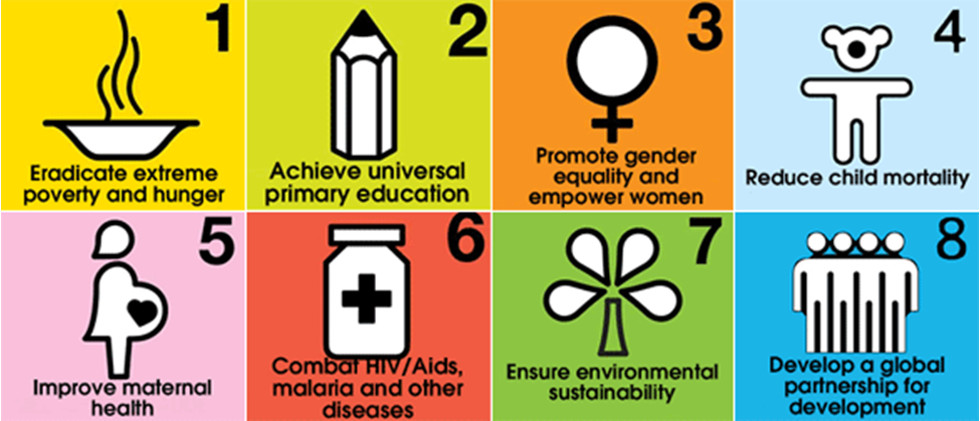
\includegraphics[width=\textwidth]{../img/millenniumdoelstellingen.jpg}
	\caption{De 8 millenniumdoelstellingen \autocite{NOS2015}}
	\label{milleniumdoelstellingen}
\end{figure}

 \subsubsection{ICT binnen de millenniumdoelstellingen}
 Op het eerste zicht is geen enkele doelstelling specifiek gericht op ICT. ICT kan bij vele doelstellingen een hulpmiddel zijn om die doelstelling te bereiken. Zo kon onder de achtste doelstelling "wereldwijde samenwerking", ICT een concretere functie innemen: ICT kan ervoor zorgen dat landen, en personen sneller kunnen communiceren. Het was een uitdaging, om in functie van wereldwijde samenwerking, ICT een boost te geven. Het gaat onder andere om ontwikkeling op vlak van internetaansluitingen, mobiele telefoons en andere ICT gerelateerde zaken. \autocite{NOS2015}
 
\subsubsection{Algemene resultaten}
De landen die zich engageerden hadden 15 jaar de tijd om de doelstellingen te behalen. Op 31 december 2015 liepen de doelstellingen af.
Een aantal doelstellingen had een positieve afloop, en bereikten hun vooropgestelde doel. Zo gaan bijna evenveel meisjes als jongens naar school, hebben meer mensen toegang tot drinkbaar water dan ooit en werd de extreme armoede gehalveerd. Ook op vlak van basisonderwijs, de strijd tegen hiv/aids en het terugdringen van kinder- en moedersterfte werd vooruitgang geboekt. Maar de vooruitgang van deze laatste doelstellingen was niet voldoende om de vooropgestelde doelen te behalen. \autocite{Tierens2014}

Deze resultaten zijn erg algemeen. Er wordt gesproken over algemene vooruitgang, en niet over welke landen of continenten meer vooruitgang boekten dan anderen. Zo boekte China een spectaculaire vooruitgang, maar hinken de regio's Sub-Sahara Afrika en West-Azië zwaar achterop. \autocite{Tierens2014}
 
 \subsubsection{Resultaten op vlak van ICT}
Over de vooruitgang op vlak van informatica stelt \autocite{Kampherbeek2012} het volgende: "Het aantal mobiele telefoons en internet aansluitingen is de laatste jaren ook in de ontwikkelingslanden flink gestegen. Doordat er meer mensen in ontwikkelingslanden wonen dan in ontwikkelde landen is het aantal unieke internetgebruikers nu groter in ontwikkelingslanden dan in de ontwikkelde landen. Desondanks is de kloof met de ontwikkelde landen procentueel op dit gebied nog groot. In 2010 lag het aantal internetgebruikers in de ontwikkelingslanden op 21 per 100 inwoners (en in de minst ontwikkelde landen slechts 3 per 100). In de rijke landen waren dat er in 2010 gemiddeld 72 op de 100 inwoners."
 
 \subsubsection{Kritiek op de millenniumdoelstellingen}
 Volgens  \autocite{VN2015} werden ommige doelstellingen onvoldoende ambitieus geformuleerd. Bovendien hield men geen rekening met nijpende 'nieuwe' problemen zoals ecologie of ongelijkheid. Ook werden vaak problemen aangepakt die typisch waren aan ontwikkelingslanden. Problemen zoals het behouden van levenskwaliteit of ecologische duurzaamheid waren namelijk ook voor ons land zeer relevant. Nog kritiek op de MDGs kwam er, omdat de VN elke doelstelling apart beschouwde, in plaats van het volledige plaatje te bekijken. \autocite{VN2015}
 % ELLEN: Wat beperkt weergegeven. Belangrijk om aan te geven, aangezien dit zorgde voor de overgang naar de SDG’s die veel ruimer waren en waarbij een volledig andere aanpak werd voorzien. Zie ook verder.

\subsection{Sustainable Development Goals}
Nadat de millenniumdoelstellingen verliepen koos men voor een andere aanpak. Er was nood aan nieuwe doelstellingen, maar die dienden op andere manieren geformuleerd worden. Door de eerder besproken tekortkomingen van de MDG's moesten de niewe doelstellingen nu onder andere ook relevant voor alle landen in de wereld, en zo kwamen de SDG's tot leven.  \autocite{VN2015}

De Sustainable Development Goals, in het kort, de SDG's, zijn een set van duurzame ontwikkelingsdoelstellingen die van de wereld een betere plaats moeten maken. De SDG’s zijn een oproep tot actie voor alle landen, zo wel arme en rijke, om welvaart te bevorderen en tegelijkertijd de planeet te beschermen tegen klimaatverandering. Ze leggen de grondslag voor het beëindigen van armoede, met strategieën die zowel economische groei ontwikkelen als een reeks sociale behoeften aanpakken, zoals onderwijs, gezondheid, sociale bescherming en werkgelegenheid. \autocite{VerenigdeNaties2004}

% Ellen Best ook ergens uitleggen dat de SDG’s de Milleniumdoelstellingen opvolgen en breder gaan dan deze (zie kritieken milleniumdoelstellingen). Ook de aanpak is deze keer anders (niet enkele op niveau van wereldleiders, maar gericht op actieve participatie van alle bevolkingslagen). Kijk even of je hier nog wat over kan vinden om kort toe te voegen, dus link/overgang Milleniumdoelstellingen en SDG’s.

De SDG's werden in september 2015 aanvaard door de wereldleiders, die de Agenda 2030 voor duurzame ontwikkeling goed keurde. UNDP werkte aan het versterken van nieuwe kaders voor ontwikkeling, rampenrisicovermindering en klimaatverandering. Ze ondersteunde de inspanningen van landen om de duurzame ontwikkelingsdoelen van mondiale doelen te bereiken, die de globale ontwikkelingsplannen tot 2030 zullen sturen.

De SDG's gingen in 2016 van kracht en gelden tot 2030. Ze vervangen de eerder besproken millenniumdoelstellingen. Er werden 17 doelstellingen opgesteld, die op 1 januari 2016 in werking traden. \autocite{DevelopmentProgram2020}
 
 \subsubsection{De verschillende doelstellingen}
 \begin{enumerate}
 	\item Geen armoede
 		\item Geen honger
 		\item Goede gezondheid en welzijn
 		\item Kwaliteitsonderwijs
 		\item Gendergelijkheid
 		\item Schoon water en sanitair
 		\item Betaalbare en duurzame energie
 		\item Waardig werk en economische groei
 		\item Industrie, innovatie en infrastructuur
 		\item Ongelijkheid verminderen
 		\item Duurzame steden en gemeenschappen
 		\item Verantwoorde consumptie en productie
 		\item Klimaatactie
 		\item Leven in het water
 		\item Leven op het land
 		\item Vrede, justitie en sterke publieke diensten
 		\item Partnerschap om doelstellingen te bereiken
 \end{enumerate}
\autocite{VerenigdeNaties2004}

In Figuur \ref{SDGs} worden de doelstellingen duidelijk weergegeven.
 
 \begin{figure}[h!]
 	\includegraphics[width=\textwidth]{../img/SDG.jpg}
 	\caption{De 17 Sustainable Development Goals \autocite{VerenigdeNaties2004}}
 	\label{SDGs}
 \end{figure}

\subsubsection{MDG's Versus SDG's}
Hoewel men armoedebestrijding nog steeds als een overkoepelende doelstelling beschouwd, is een belangrijk verschil tussen de SDGs en de  MDGs dat men erkent dat armoede een zeer multidimensionaal probleem is. Na de kritiek op de MDGs dat de VN elke doelstelling apart beschouwde, zorgde men dat dit bij de SDG's niet het geval is. Om alle doelstellingen te halen, zal men dus rekening moeten houden hoe de doelstellingen op elkaar inwerken. Een ander belangrijk verschil met de MDGs, is dat, door dat er bij de SDGs te werd gekozen voor een veel bredere aanpak zijn de nieuwe doelstellingen nu relevant voor alle landen in de wereld. \autocite{VN2015}

\subsubsection{SDG's en ICT}
Aangezien technologische innovatie wordt erkend als de belangrijkste drijfkracht achter sociaaleconomische groei, kan het ook een cruciale rol spelen bij het ondersteunen van het succesvol uitvoeren van de duurzame ontwikkelingsdoelen (SDG's) van de Verenigde Naties. ICT heeft het potentieel niet-geautomatiseerde taken op te schalen en te versnellen in een breed scala van geavanceerde technologieën in alle sectoren. Het kan de kosten van dienstverlening verlagen, waardoor landen met lage inkomens belangrijke ontwikkelingsmijlpalen kunnen bereiken en tegelijkertijd bijdragen aan een groeiende economie en sociaal welzijn. \autocite{Ameyed2018}

\subsubsection{VN: ITU}
ITU is het gespecialiseerde bureau van de Verenigde Naties voor informatie- en communicatietechnologieën (ICT). ITU zet zich in om alle mensen ter wereld te verbinden, waar ze ook wonen en wat hun middelen ook moge zijn. Door hun werk beschermen en ondersteunen ze ieders recht om te communiceren.
Het is vanzelfsprekend dat ITU de SDG's steunt op vlak van informatica. Ze doen dat onder de hashtag \#ICT4SDG. \autocite{ITU2015}

Op hun website vullen ze voor elke SDG in wat ICT kan beteken, om dat specifiek doel te realiseren. Zo stellen ze over de SDG rond het uitroeien van hongersnood, dat ICT boeren kan helpen om de gewasopbrengsten en de bedrijfsproductiviteit te verbeteren door betere toegang tot marktinformatie, weersvoorspellingen, trainingsprogramma's en andere online informatie te creëren. \autocite{ITU2015}

Over kwaliteitsonderwijs wordt het volgende geschreven: ICT zorgt voor een revolutie in digitaal leren. Die revolutie is één van de snelst groeiende industrieën ter wereld geworden. Met mobiele apparaten hebben studenten nu altijd en overal toegang tot leermiddelen. Ook docenten gebruiken mobiele apparaten voor allerlei zaken: van alfabetisering en numerieke training tot interactieve bijles. Mobiel leren heeft inderdaad de kracht om te helpen economische barrières te doorbreken, het verschil tussen platteland en stad weg te werken, en de kloof tussen mannen en vrouwen weg te nemen. \autocite{ITU2015}

% ELLEN: Kan je verder nog zaken terugvinden over ICT en de ontwikkelingsdoelstellingen? Wordt er gesproken van het belang van ICT in het onderwijs, de digitale gap, ...? Op welke manier worden mensen nog achtergesteld indien ze geen toegang hebben tot technologische apparaten, internet e.d.

Ook bracht ITU een ''\#ICT4SDG-Toolkit'' uit. Dat zijn hulpmiddelen die ontworpen zijn om belanghebbenden te ondersteunen bij hun werk meer specifiek ter bevordering van de cruciale rol van ICT, om de vooruitgang in de richting van de doelstellingen van de Verenigde Naties voor duurzame ontwikkeling en de Agenda 2030 te bevorderen. \autocite{ITU2015}
 
\section{Het Peruviaanse onderwijssysteem}
\subsection{Basis- en voortgezet onderwijs}
Het lager en algemeen vormend, voortgezet onderwijs (educación básica regular) is opgedeeld in 3 fases:
 \begin{itemize}
\item Educación inicial (peuter- en kleuteronderwijs), leeftijdscategorie 0 tot 2 en 2 tot 5 jaar
\item Educación primaria (basisonderwijs), leeftijdscategorie 6 tot 11 jaar
\item Educación secundaria (voortgezet onderwijs), leeftijdscategorie 11/12 tot 16/17 jaar.
\end{itemize}
Er wordt een onderscheid gemaakt tussen openbare en particuliere scholen: een openbare school is een staatsschool, en is gratis. Er is toegang voor alle kinderen. Een private, of particuliere school is betalend. Voor zowel de openbare als de private scholen is een nationaal curriculum vastgesteld.  \autocite{Nuffic2015}

In het algemeen geldt dat de kwaliteit van het private onderwijs hoger ligt dan het privé onderwijs

%todo Hoe staat het met de kwaliteit bij beide types van onderwijs? Probeer het verschil toch iets uitgebreider toe te lichten... Hier is het zeker heel erg zinvol om een keer met Sadith uit te wisselen

Het peuter- en kleuteronderwijs omvat 5 lesuren per dag, 25 uur week en minimaal 900 uur per jaar. Het basisonderwijs (educación primaria) bestaat uit 6 lesuren per dag, 30 uur per week en ten minste 1100 uur per jaar. Het voortgezet onderwijs omvat 7 lesuren per dag, 35 uur per week en minimaal 1200 uur per jaar. \autocite{Nuffic2015}

Het voortgezet onderwijs wordt afgesloten met het getuigschrift ''Certificado Oficial de Estudios''. Dit getuigschrift geeft in Peru toegang tot de toelatingsexamens van het hoger onderwijs. Voor de meeste universiteiten is naast het middelbare schooldiploma tevens een toelatingsexamen vereist. De precieze toelatings- en registratieprocedures zijn opgenomen in het statuut van de universiteit. De toelatingsexamens vinden doorgaans 1 à 2 keer per jaar plaats in de vakantieperiode. \autocite{Nuffic2015}

\subsection{Hoger onderwijs}
\subsubsection{Universidades}
 "Universidades" bieden wetenschappelijke en technologische onderzoeks-programma’s aan tot en met het doctoraat, alsmede hoger beroepsgerichte opleidingen. Het academisch jaar heeft een minimale duur van 34 weken en vangt op zijn laatst aan op de eerste werkdag van de maand april van elk jaar. Opleidingen worden doorgaans opgedeeld in semesters en aan de vakken van het curriculum worden créditos (studiepunten) toegekend. \autocite{Nuffic2015}
 
 \subsubsection{Institutos y escuelas de educación superior }
Institutos en escuelas de educación superior zijn instellingen die lijken op het belgische beroepsonderwijs. Ze geven studenten de mogelijkheid om te studeren voor een specifiek beroep. Zo bestaan er 'Institutos y escuelas de educación superior pedagógicos' en 'Institutos y escuelas superiores de formación artística' waar er kan gestudeerd worden om respectievelijk leerkracht en kunst leerkracht te worden. Ook bestaat er een technische varianten, 'Institutos y escuelas de educación superior tecnológicos', waar men allerlei technische richtingen kan volgen. \autocite{Nuffic2015}
% ELLEN: Naast de universidades bestaan er ook institutos de educación superior, vergelijkbaar met bij ons in België de hogescholen. Deze opleidingen zijn vaak eerder technisch van aard of minder zwaar dan de opleidingen aan de universidades. Ik zou hier kort nog wat over toevoegen.


\subsection{Beoordelingssystemen}
In zowel het hoger als voortgezet onderwijs wordt een cijfersysteem gehanteerd van 0 (laagst haalbare cijfer) tot 20 (hoogst haalbare cijfer), met 11 als voldoende. De leerlingen in het lager en voortgezet onderwijs worden gequoteerd met letters: C (onvoldoende), B (Voldoende), A (Goed), AD (Zeer goed). \autocite{Nuffic2015}

\subsection{kwaliteit van het onderwijs}
De kwaliteit van het onderwijs verschilt van land tot land. \autocite{Review2020} De website 'World Population Review' stelt dat over het algemeen mensen in onderontwikkelde landen helemaal geen toegang hebben tot kwaliteitsvol onderwijs. 
In een onderzoek van de  Universiteit van Pennsylvania \autocite{UsNews2020} werden 20.000 mensen ondervraagt, om hun landen te vergelijken op basis van allerlei parameters, waaronder onderwijs. In het onderzoek werden 4 scores voorzien: Een totale score, een score op het leesniveau van leerlingen, een wiskunde score en een wetenschapsscore. De scores liggen telkens tussen 1000 en 1800. België heeft een totaalscore van 1528. De lees score bedraagt 506, de wiskundescore 515 en wetenschapsscore van 507. Peru heeft een totaalscore van 1104, een leesscore van 370, een wiskunde score van 365 en een wetenschapscore van 369. In de rangschikking van alle 63 deelnemende landen staat Belgie 15de, en Peru op der voorlaatste, 62ste plaats.


% ELLEN: Ik mis nog wat informatie over het onderwijs in Peru. - Hoe is het gesteld met de kwaliteit, waar ze staan ze hier? 
% Zijn er hiaten in het onderwijssysteem? Kritieken?
% -> ik zou dan vooral naar het staatsonderwijs kijken omdat het hier gaat over de verantwoordelijkheid van de Peruviaanse regering en Peru als land omtrent onderwijs.
%todo Wordt ICT voorzien in het officiële leerplan vanuit het Ministerie van Onderwijs? Zijn er hier voldoende middelen voor in de scholen? Zijn de leerkrachten hier voldoende op voorbereid? Is ICT voorzien in de lerarenopleidingen?...

%todo Hier moet dus zeker en vast nog een onderverdeling komen over ICT in het onderwijs in Peru. Hoe wordt ICT ingezet binnen educatie? (en eventueel volgende titel/ondertitel dan aanpassen zodat deze hier logisch op aansluit.)

\subsection{ICT en onderwijs}
Op 25 juli 2019 kondigde de toenmalige Peruviaans minister Flor Pablo aan dat in 2021 alle stedelijke onderwijsinstellingen verbonden zullen zijn met het internet en zullen beschikken over digitale apparatuur. Dat deed ze tijdens STEAM 2019, een gratis internationaal Seminarie rond het onderwijs en de cultuursector, dat als doel heeft de kwaliteit van het onderwijs te verbeteren door transformatie en innovatie. Ook vertelde ze toen dat in de huidige situatie 60\% van de onderwijsinstellingen geen adequate technologische uitrusting heeft, 79\% van de onderwijsinstellingen geen toegang tot het internet heeft, 55\% van de leraren geen vaardigheden heeft om de digitale technologieën te gebruiken en 64\% van de kinderen blootgesteld wordt aan cyberrisico's. \autocite{Ministerio de Educación}

\section{ICT in peru}
\subsection{Digital gap}
De mogelijkheid om toegang te krijgen tot computers en internet wordt steeds belangrijker om jezelf volledig onder te kunnen dompelen in de economische, politieke en sociale aspecten van de wereld. Het idee van de "digitale kloof" verwijst naar de groeiende kloof tussen de kansarme leden van de samenleving, vooral het arme, landelijke, bejaarde en gehandicapte deel van de bevolking dat geen toegang heeft tot computers of internet; en de rijke, middenklasse die het zich wel kan veroorloven. De digital gap kan bekeken worden van individu tot individu, maar ook op groter globaal niveau. \autocite{Marichick2000}

Volgens de wereldbank had in 2018 88.7\% van de Belgische bevolking toegang tot het internet, wat erg veel is. In Peru had op dat moment 52.5\% van de bevolking toegang tot het internet. In de hele wereld was dat 49.7\%. \autocite{WereldBank2018}

\subsection{One laptop per child}
Om deze digital gap kleiner te maken was er in 2005 een project genaamd One Laptop Per Child (OLPC). De naam zegt het zelf: het doel was om voor elk kind (kinderen in ontwikkelingslanden) een educatieve computer te voorzien. De visie was educatieve kansen creëren voor 's werelds armste kinderen door elk kind een robuuste, goedkope, energiezuinige, verbonden laptop te bieden met inhoud en software die was ontworpen voor samenwerkend en zelf-bekrachtigd leren. Wanneer kinderen toegang hebben tot dit type hulpmiddel, zouden ze betrokken raken bij het eigen onderwijs. Ze leren, delen, creëren en werken samen. Ze raken verbonden met elkaar, met de wereld en met een betere toekomst. \autocite{OneLaptopPerChild2005}

Zelf zegt OLPC dat ze geen laptopproject zijn, maar een onderwijsproject. De kleine groene, XO-laptop kostte (slechts) 100 Amerikaanse Dollar. De laptops hadden een op Linux gebaseerd besturingssysteem, Sugar OS. Sugar OS is gebouwd op Red Hat Linux, en het open-source ontwerp zou kinderen volledige toegang tot de computer geven. De kinderen zouden kunnen rondneuzen in de kernfirmware van de laptop. OLPC zou naar verluid een aanbod van gratis Mac OS X-licenties van Steve Jobs hebben afgewezen. \autocite{Robertson2018}

Na het eerste prototype werden nog een aantal dingen veranderd. Het resultaat was een opvallend ogende machine die bekend staat als de XO-1: een speelse groen-witte laptop met afgeronde randen, een draaibare 'nek' in plaats van een standaardscharnier en een dikke rand rond het 7,5-inch scherm. Ook had de computer een vouw-toetsenbord. Oorachtige antennes klapten omhoog om het Wi-Fi-bereik uit te breiden. Zie Figuur \ref{xo-1}. \autocite{Robertson2018}

 \begin{figure}[h!]
	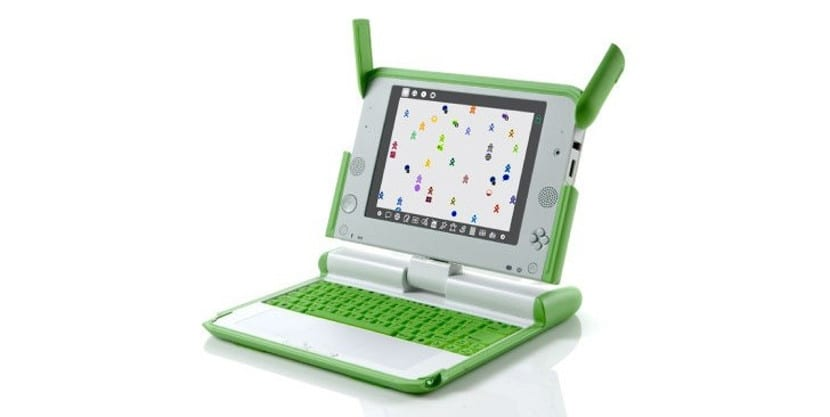
\includegraphics[width=\textwidth]{../img/olpc-xo-1.jpg}
	\caption{OLPC: XO-1}
	\label{xo-1}
\end{figure}

Echter: door een samenloop van omstandigheden mislukte het project. Achteraf gezien was 100 dollar iets te optimistisch. De fabrikanten dienden de prijs met 30 dollar te verhogen, en de laptop werkte nauwelijks. De prijs steeg uiteindelijk tot ongeveer 180 dollar, en zelfs \textit{toen} had het ontwerp nog grote afwijkingen. De laptops gingen ook veel sneller stuk dan eerst gedacht. Het project kreeg zowel veel lof als veel kritiek. Zo werd bovendien vaak gezegd dat het project voldeed aan een behoefte die er eigenlijk niet was. Vele landen en gemeenschappen hadden op dat moment andere behoeften dan kleine kindercomputers. \autocite{Robertson2018}

\subsubsection{OLPC in Peru}
Het grootste OLPC-programma tot nog toe vond plaats in Peru volgens \autocite{Trucano2012}. Vele OLPC-supporters beweren dat OLPC zijn eerste grootschalige test in2007 in Peru had. Er zouden 902.000 educatieve computers aangekocht zijn door de Peruviaanse regering. Echter werd het programma geteisterd door logistieke problemen. De machines werden naar de scholen verzonden met slechte elektrische stroomkabels en leraren kregen weinig ondersteuning of training. \autocite{Robertson2018}

Pablo Ibarrarán onderzocht samen met een team van onderzoekers de resultaten van de invoering van OLPC in Peru. \autocite{Ibarraran2012} Ze deden een evaluatie van het project op vlak van educatie. Hun focus lag vooral op academische prestaties op vlak van wiskunde en taal. Het verbeteren van deze vakken was de doelstelling van het gehele OLPC project. Ook deden ze een cognitieve vaardigheidstest, een verbale vlotheidstest en een programmeertest. Dit deden ze via een gerandomiseerde controleproef. Er werden 210 scholen geselecteerd uit een groep van 320 scholen. Deze scholen ontvingen laptops, terwijl de andere scholen dat niet deden. De scholen waren vóór het programma identiek en behalve de computers verschilde er niets tussen hen. Dat zorgde ervoor dat de onderzoekers er vrij zeker van waren dat elk verschil na het programma kan worden toegeschreven aan OLPC. \autocite{Ibarraran2012}

De resultaten waren opvallend: eerst en vooral heeft het programma de toegang tot computers drastisch verbeterd. Er waren 1,18 computers per leerling in de behandelde groep, vergeleken met 0,12 in controle scholen. 82\% procent van de behandelingsstudenten meldde de afgelopen week een computer op school te hebben gebruikt, vergeleken met 26\% in de controlegroep. Ook gaf 42\% van de behandelingsstudenten aan de afgelopen week thuis een computer te hebben gebruikt, tegenover 4 procent in de controlegroep. \autocite{Ibarraran2012}

Naast deze resultaten op vlak van ICT vond men dat er geen bewijs was dat het programma het niveau van wiskunde of taal van de kinderen had verbeterd. Dat zou kunnen komen omdat de laptops niet specifiek in de leerplannen waren opgenomen, en de computers ook geen specifieke wiskundige of taalsoftware bevatten. Ook had het programma geen invloed de tijd die besteed werd aan het maken van huiswerk, noch verhoogde het de kwaliteit of motivatie om het huiswerk te maken. In het algemeen stelde het onderzoek dat de kwaliteit van het onderwijs niet werd beïnvloed, wat toch een hard verdict was voor een project dat zichzelf geen laptop project, maar educatie project noemde. \autocite{Ibarraran2012}

\subsection{PeruEduca}
Sinds 2011 is PeruEduca een nationaal, digitaal leerplatform dat educatieve tools, diensten en middelen biedt aan leraren, studenten en ouders. Het systeem heeft als doel ruimte te creëren voor het beheer van kennis, onder meer door samen te werken en ervaringen uit te wisselen. \autocite{EducationPeru2020}

Zo verplichte het ministerie van onderwijs tijdens de recente uitbraak van het covid-19 virus alle leraren in Peru om zich te registreren en een verplichte virtuele cursus tegen het virus te volgen. \autocite{Educacion2020}


%todo Wat is nu de stand van zaken op dit moment omtret de toegang tot ICT in Peru in het staatsonderwijs of binnen educatie? Kan je hier gegevens over terugvinden? Welke noden zijn er (nog steeds)? + besluit van dit hoofdstuk.
%todo -> van hieruit kunnen pas je suggesties komen tot optimalisatie. (Kijk nog eens terug naar je BP voorstel!)



%%=============================================================================
%% Methodologie
%%=============================================================================

\chapter{Methodologie}
\label{ch:methodologie}

%% TODO: Hoe ben je te werk gegaan? Verdeel je onderzoek in grote fasen, en
%% licht in elke fase toe welke stappen je gevolgd hebt. Verantwoord waarom je
%% op deze manier te werk gegaan bent. Je moet kunnen aantonen dat je de best
%% mogelijke manier toegepast hebt om een antwoord te vinden op de
%% onderzoeksvraag.

Om een duidelijk beeld te krijgen van de stand van zaken van het onderwijs in Peru en hoe informatica er zijn weg vindt in het onderwijs werd ervoor gekozen om verschillende specialisten te interviewen. De specialisten hebben door studies en ervaring veel relevante kennis, elk binnen hun eigen domein. Ze werden gekozen om vanuit verschillende invalshoeken een zicht te krijgen op de problematiek. Er werden gelijkaardige vragen gesteld om de verschillen en gelijkenissen tussen de ervaringsdeskundigen bloot te leggen en duidelijk weer te geven.

De vragen die tijdens de verschillende interviews werden gesteld, zijn onder te verdelen in 4 grote onderwerpen: 

\begin{itemize}
	\item De informatica-infrastructuur op scholen
	\item Het toepassen van informatica in de lessen
	\item De informatica leerkracht op school
	\item Hoe gaat Peru om met informatica in het algemeen?
\end{itemize}

Na de interviews worden de uitspraken, gedaan door de geïnterviewde, gecontroleerd en gestaafd of weerlegd met reeds vergaarde bronnen uit de literatuurstudie en nieuwe bekomen informatie. Hierna volgt een conclusie met suggesties tot optimalisatie.


%%=============================================================================
%% InterviewSadith
%%=============================================================================

\chapter{Interview met Sadith Van Añañau ORG}
\label{ch:interviewMetSadith}

%% TODO: Hoe ben je te werk gegaan? Verdeel je onderzoek in grote fasen, en
%% licht in elke fase toe welke stappen je gevolgd hebt. Verantwoord waarom je
%% op deze manier te werk gegaan bent. Je moet kunnen aantonen dat je de best
%% mogelijke manier toegepast hebt om een antwoord te vinden op de
%% onderzoeksvraag.
\section{Inleiding}
Om een antwoord te kunnen bieden op de eerst onderzoeksvraag, werd ervoor gekozen om een interview af te nemen met Sadith Paez Montesinos. Sadith is één van de oprichtsters van Añañau. Añañau is een non-profit en niet-gouvernamentele organisatie die in december 2014 werd opgericht in Cusco, Peru. De organisatie werkt met kinderen en jongeren tussen 4 en 18 jaar oud die in situaties van extreme armoede en onstabiele familiesituaties leven in het district San Jeronimo, een buitenwijk van Cusco. Sinds januari 2015 is de organisatie als officiële NGO erkend in Peru. Omdat ze geloven in de kracht van goed en inclusief onderwijs als springplank naar een betere toekomst, is Añañau in de eerste plaats een educatief project. Via huiswerkbegeleiding en spelend leren stimuleert Añañau de ontwikkeling van de kinderen en trachten ze nieuwe kansen te creëren. \autocite{Ananau2020}

Door haar ervaring in het werkveld beschikt Sadith over relevante info omtrent het onderwijs in Peru. 

\section{Interview}
\textbf{Hebben de meeste staatsscholen in Peru computers ter beschikking op school? Welke apparatuur is er? Zijn er gebreken aan deze apparatuur? Is de apparatuur bruikbaar?}

\textit{Sadith:} Niet alle scholen hebben computers. Van de scholen die zich in de binnenstad bevinden heeft volgens mij 80\% van de scholen computers ter beschikking. Bij de scholen buiten de stad, in het binnenland van Peru is dat volgens mij 40\% van de scholen. Als een school dan computers heeft, zijn dat er ongeveer 10 of 20 computers per 200 leerlingen.

\textbf{Hoe gebruiken de kinderen de computers om te leren?}

\textit{Sadith:} Normaal gezien gebruiker ze de computers om computer les te krijgen. De leerlingen gaan dus niet voor andere vakken aan de slag met informatica. 

\textbf{Wat leren de kinderen dan tijdens de computerlessen?}

\textit{Sadith:} Ze leren specifieke programma's gebruiken. Ze leren niet programmeren, maar leren vooral praktisch werken met bijvoorbeeld Word en Excel.

\textbf{Passen de staatsscholen informatica binnen hun curriculum nog op andere manieren toe, zoals met smartborden of tablets?}

\textit{Sadith:} Smartborden hebben de scholen niet. Ongeveer 5 jaar geleden werd een project opgestart waarbij tablets op scholen gestimuleerd werden. De tablets werkten in de grote steden, maar in het binnenland was er meestal geen verbinding. Hier in Peru moeten we elke 5 jaar gaan stemmen en verandert de regering. Het komt vaak voor dat nieuwe regeringen andere aanpakken hebben, en niet meer in deze projecten willen investeren. Na de verandering van de regering werd het tablet project stop gezet.

Nu sinds kort, zitten we in de huidige covid-19 crisis. Daardoor investeert de overheid op dit moment graag in ICT projecten voor het onderwijs, omdat alle leerlingen thuis moet blijven, en thuis moet studeren. Onlangs kochten ze volgens mij nog 13.000 computers aan die zich via satellieten kunnen verbinden met het internet. Deze computers zouden dienen om aan studenten uit te delen, zodat ze thuis zelf op de computer voor school kunnen werken. 

\textbf{Moeten kinderen die naar staatsscholen gaan soms huiswerk maken op computers? Wat moeten ze doen als ze geen computer hebben?}

\textit{Sadith:} Ja, de kinderen moeten thuis huiswerk maken op computers. Ze krijgen huiswerk op de computer van al hun vakken. Als ze thuis geen computer hebben gaan ze naar een internetcafé. Daar kunnen ze computers gebruiken voor 1 sol per uur (ongeveer 0,25 eurocent) en printen. Hier in Peru zijn er veel internetcafés. Een nadeel is wel dat de kinderen er vaak in aanraking komen met videospelletjes. Ze worden verleid, zijn vaak afgeleid, en komen niet aan huiswerk maken toe. 

\textbf{Zijn de leerkrachten voldoende opgeleid om computers te gebruiken?}

\textit{Sadith:} Niet alle leerkrachten kunnen met computers werken. Dit is een groot probleem hier. Er zijn leerkrachten die al veel ervaring hebben, en bijna op pensioen gaan. Deze generatie leerkrachten heeft veel minder voeling met de nieuwe technologieën.

\textbf{Zijn er dan geen bijscholingen voor die leerkrachten?}

\textit{Sadith:} Voor informatica moeten de leerkrachten zichzelf bijscholen. Dit wordt niet georganiseerd door de overheid. Er wordt dus verwacht dat de leerkrachten zelf op zoek gaan, en ervoor zorgen dat ze zelf op de hoogte zijn. In de relativiteit loop dit dus vaak fout en zijn er leerkrachten waarvan de computerkennis heel erg beperkt is. Wel bestaan er platformen die lessen geven. Die lessen zijn voor alle inwoners, en niet specifiek gericht op lesgevers.

\textbf{Zijn er ICT-leerkrachten, en zijn ze opgeleid?}

\textit{Sadith:} Hier in Cusco kan je volgens mij niet studeren voor ICT leerkracht. Vaak worden ICT leerkrachten aangesteld die ofwel gewoon veel weten van ICT, en hiervoor dus niet opgeleid zijn of er worden ICT specialisten gezocht die les willen geven, maar dat is heel erg duur en vaak onbetaalbaar.

\textbf{Is er programmatuur die kan gebruikt worden op de computers door de kinderen, zoals een taal- of rekenprogramma?}

\textit{Sadith:} Hier in Cusco kan je volgens mij niet studeren voor ICT leerkracht. Vaak worden ICT leerkrachten aangesteld die ofwel gewoon veel weten van ICT, en hiervoor dus niet opgeleid zijn of er worden ICT specialisten gezocht die les willen geven. Meestal willen de specialisten geen les geven, en kunnen ze meer verdienen door ergens anders aan de slag te gaan. Als een school er dan toch voor kiest om een specialist in dienst te nemen moeten ze veel betalen en is dit meestal onbetaalbaar.
	
\textbf{Zijn er digitale omgevingen waarop kinderen kunnen aanloggen?}

\textit{Sadith:} Vroeger niet, nu sinds een maand is de overheid begonnen met het ontwikkelen van een platform. Door de recente uitbraak van het covid-19 virus voorziet de overheid een platform waarop kinderen van thuis uit kunnen les volgen. Het platform heet aprendo en casa (https://aprendoencasa.pe/). Natuurlijk bereikt het platform alleen kinderen die toegang hebben tot een computer met internet. Verder worden er nu ook lessen uitgezonden op de radio, en televisie kanalen voor de overheid. Elke leeftijdsgroep heeft een tijdsspanne waarop ze dagelijks lessen kunnen volgen. Een specifiek platform voor elke school, waarop de leerlingen kunnen inloggen bestaat naar mijn weten niet. 

Op dit moment, door de pandemie, proberen leerkrachten vooral contact te houden met hun leerlingen via WhatsApp-groepen.

\textbf{Wat zijn de knelpunten op vlak van informatica in het onderwijs in Peru? Hoe kunnen deze knelpunten weggewerkt worden?}

\textit{Sadith:} Volgens mij zijn er 3 grote problemen: eerst en vooral was educatie geen prioriteit voor de regeringen in het verleden. Ze investeerden niet echt in scholen en educatie. Als er nieuwe scholen werden gebouwd, was er meestal geen budget meer vrij om computers aan te schaffen. Als de regeringen al investeert in educatie, zagen ze liever mooie gebouwen, dan computers op scholen. Volgens mij is geld dus de hoofdreden. Verder is vooral de infrastructuur een groot probleem. Vele scholen buiten de stad hebben geen internet aansluiting, door de moeilijke ligging, en de bergachtige geografie van Peru. Door alle bergen is het vaak heel gecompliceerd, en moeten particulieren zelf antennes aanschaffen om op internet te kunnen. Voor scholen zijn er dus veel kosten, en daar hebben ze meestal geen geld voor. Daardoor zijn computers onnuttig, omdat ze niet functioneel zijn. De huidige regering doet zijn best om ICT bij kinderen op scholen te ondersteunen. Zoals ik al zei kochten ze al grote aantallen computers voor aan de kinderen die geen toegang hebben tot informatica te geven.

Het tweede probleem is, zoals ik al zei, dat telkens als de regering wijzigt er een ander plan van aanpak is. Soms zijn er heel goede projecten die bij een regeringswissel gestopt worden. Zo ken een regering dus 5 jaar lang een project opzetten en kan de volgende regering te niet doen, wat erg jammer is. 

Het laatste probleem is dat er weinig informatica leerkrachten zijn, zoals ik eerder uitlegde. Er is hier in Cusco geen opleiding, en specialisten zijn erg duur.

Een oplossing zou kunnen zijn om, zoals wij doen op het project Añañau, krachten van mensen te bundelen en samen te zoeken naar budgetten waarmee er doelen kunnen bereikt worden. 

\textbf{Hoe komt het dat Peru niet verder staat op vlak van informatica, wat liep er fout in het verleden?}

\textit{Sadith:} Vaak is corruptie een probleem geweest in het verleden volgens mij. De huidige regering heeft de aankoop van computers voor op scholen duidelijk geprioriteerd, maar vroeger was dat niet het geval. Regeringen probeerden vaak geld in eigen zak te steken, en dat liep helemaal fout. 
 
\subsection{Besluit}
% combinatie met literatuur
% nog een interview?

Sadith haalde tijdens het gesprek aan dat de overheid recentelijk vele computers aankocht die verbinding maken met een sateliet om op verbinding met het internet te kunnen maken. Op 18 april verspreidde het ministerie van onderwijs een persbericht waarin ze vertelden dat ze 840.000 tablets aankochten met mobiel internet voor schoolkinderen in afgelegen landelijke en stedelijke gebieden. Dit, zodat ze de kinderen kunnen blijven studeren en de digitale kloof kan worden verkleind. Op deze manier kunnen de kinderen onderwijs vanop afstand volgen.\autocite{Minedu2020} Nadat ik Sadith confronteerde met het persbericht zei ze me dat ze het over dit bericht had in het interview. 

%aprendo en casa 
Ook vertelt Sadith over 'aprendo en casa' (vertaald: ik leer thuis). Dat is een programma dat de regering aanbied om de schoolgaande kinderen te voorzien van thuis onderwijs. Het \autocite{Minedu2020a}
%Studeren in cusco voor ict leerkracht ?

%%==========================================================================
%% Interview Erick
%%==========================================================================

\chapter{Interview met Erick, leerkracht}
\label{ch:interviewErick}

%% TODO: Hoe ben je te werk gegaan? Verdeel je onderzoek in grote fasen, en
%% licht in elke fase toe welke stappen je gevolgd hebt. Verantwoord waarom je
%% op deze manier te werk gegaan bent. Je moet kunnen aantonen dat je de best
%% mogelijke manier toegepast hebt om een antwoord te vinden op de
%% onderzoeksvraag.
\section{Inleiding}
Erick Paez Montesinos werkte gedurende 9 jaar voor het Peruviaanse ministerie van onderwijs. Daarnaast gaf hij les in verschillende onderwijs instituten en werkte hij in een monitoraat dat andere leerkrachten op pedagogische vlak bijschoolt en begeleid. Op dit moment geeft hij geen les meer, omdat hij een andere richting uitging, maar vorig schooljaar gaf hij les in educación primaria. Dat is het Peruviaanse basis onderwijs, waar kinderen tussen 6 en 11 jaar onder vallen. \autocite{Nuffic2015} Ook gaf hij les in educación initial, educación secundaria en educación superior. Hij is iemand met veel ervaring binnen het onderwijs en kan ons relevante informatie bezorgen voor dit onderzoek. Dit interview werd, door de huidige maatregels tegen het Covid-19 virus afgenomen, vanop afstand.

 %Maestro Titular de Primaria

\section{Interview}

\textbf{In welke school werkte je?}

\textit{Erick:} Ik werkte in een staats school in Apurímac. Dat is niet in Cusco, maar een regio daarbuiten. Daar werkte ik in instituut 50640, genaamd Sagrado corazon de Jesus.
%http://www.dreapurimac.gob.pe/inicio/images/ARCHIVOS_2019/CD-19/CD-2019-UGEL-COTABAMBAS.pdf

\textbf{Hoeveel leerlingen zitten er gemiddeld in de klassen waarin u lesgaf?}

\textit{Erick:} Er zitten normaal gezien 20 tot 25 leerlingen in elke klas. Op de hele school waren er 11 klassen, dus er waren ongeveer 220 tot 250 leerlingen op de school waar ik les gaf. %5:06

\textbf{Had je op jouw school computers ter beschikking? Welke apparatuur was er? Waren er problemen met deze apparatuur?}

\textit{Erick:} Er was 1 computerklas die gebruikt kon worden door leerkrachten met hun leerlingen. Leerkrachten konden het lokaal boeken en de computers in hun les verwerken en gebruiken. Deze computers werden specifiek gebruikt voor informatica lessen. Verder had de school ook laptops die door de overheid betaald werden. Deze laptops konden door klassen uitgeleend worden, en werden gebruikt als hulpmiddel tijdens andere lessen, zoals wiskunde of taal. De laptops hebben minder rekenkracht en zijn alleen voorzien van een aantal basis functionaliteiten. Ze zijn gemaakt om educatieve programma's op te gebruiken en informatie te raadplegen op het internet. Het zijn wit-groene laptops van het merk XO. De school had ongeveer 70 laptops van dit type. Op dit moment worden ze minder en minder gebruikt, omdat ze verouderd beginnen te zijn.

\textbf{Had jouw school een ICT leerkracht?}

\textit{Erick:} Ja, onze school had een ICT leerkracht. Hij was verantwoordelijk voor het controleren, en organiseren van alles dat met ICT te maken had. Normaal gezien worden deze leerkrachten geselecteerd en opgeleid door de educatieve koepel van het onderwijs district. Ik denk dat ongeveer 85\% van de publieke scholen in Peru een ICT leerkracht heeft. Bij ons op school was dit iemand die extra lessen had gevolgd, en zich had bijgeschoold tot leerkracht informatica. In andere scholen zijn er ook ICT leerkrachten die effectief informatica gestudeerd hebben.

\textbf{In hoeverre kunnen leerkrachten die geen ICT geven als vak, om met informatica?}

\textit{Erick:} Er wordt verwacht van alle leerkrachten dat ze een basisniveau ICT hebben. Echter komt het vaak voor dat leerkrachten met veel ervaring niet goed overweg kunnen met computers. Dat komt omdat ze door de jaren heen niet voldoende bijles kregen. Er wordt verwacht dat ze zichzelf bijscholen en dat gebeurd meestal niet.

\textbf{Als leerlingen informatica les krijgen, wat leren ze dan?}

\textit{Erick:} Ze leren niet echt specifiek applicaties te gebruiken maar vooral het basis gebruik van de computer. Aan en uit zetten, iets op zoeken op het internet, .. Maar echt bijvoorbeeld in Excel leren werken of programmeren leren ze niet.

\textbf{Krijgen leerlingen huiswerk op de computer?}

\textit{Erick:} Ja, als kinderen huiswerk krijgen is dat meestal op papier, en gebruiken ze hun laptops als hulp middel. In kleine gemeenschappen, waar de mensen meestal arm zijn, en dus thuis geen computers hebben, zijn er scholen waarop de leerlingen van educación primaria hun laptops die ze op school krijgen mee naar huis mogen nemen. Daar kunnen ze via satelliet verbindingen, die gratis zijn, filmpjes kijken, dingen opzoeken en educatieve spelletjes spelen. 

\textbf{Worden de laptops dan niet gestolen? Wordt er geen misbruik gemaakt van het systeem?}

\textit{Erick:} Neen, als dat gebeurt zal de school altijd uitvoerig onderzoeken wat er gebeurde. Dit gaat om educatieve laptops, dus echt interesse is er niet naar. Een leerling kan zijn laptop dus niet verkopen, want niemand zal ze kopen. 

\textbf{Zijn er problemen met de laptops die gebruikt worden?}

\textit{Erick:} Ja, eigenlijk wel. Op de school waar ik les gaf begonnen de laptops te verouderen, daarom werden ze minder en minder gebruikt. Hun schermen waren ook niet van de beste kwaliteit en ze hadden niet genoeg geheugen capaciteit. Ook zijn de scharnieren niet sterk genoeg, en konden ze breken.

\textbf{Hoe komt het dat Peru niet verder staat op vlak van informatica, wat liep er fout in het verleden?}

\textit{Erick:} Het probleem is volgens mij groter dan informatica alleen. Vaak is de toegang tot internet beperkt in kleine gemeenschappen. Deze mensen kunnen niet op internet, en hebben ook geen financiële middelen om een computer te kunnen aankopen. Volgens mij liggen economische problemen aan de basis van het informatica probleem. Er is geen geld voor computers. Niet bij de overheid, maar vaak ook niet bij de gezinnen zelf. 

Ik denk dat NGO's kunnen helpen om deze problematieken de wereld uit te helpen en om elke school te voorzien van informatica. Ik denk dat hier in Peru er een aantal goede NGO's zijn die ons een duw in de rug gaven, en dat dit ook zou kunnen op vlak van informatica. De overheid probeert hun best te doen, om ons vooruit te helpen, maar meestal is er onvoldoende budget omdat informatica niet prioritair is. Ik denk dat, door de recente uitbraak van het covid-19 virus, de ogen van de regering open gingen. Dat blijk doordat de overheid recent veel computers aankocht om uit te delen aan kinderen, die dan op die manier vanop afstand les kunnen volgen. Ik denk dat dit misschien veel zal verbeteren aan de ondermaatse informatica kennis in het onderwijs. De staatsscholen kunnen niet zelf instaan voor de aankoop van hun computers, omdat dat dat voor hen gewoon te duur is, en omdat ze hier niet genoeg budget voor krijgen van de overheid. Nogmaals, ik denk dat de steun van NGO's veel zou kunnen betekenen.

\subsection{Besluit}
In Peru hebben alle scholen een nummer. Erick spreekt over instituut 50640. Scholen worden vaak benoemd met hun nummer in plaats van hun naam. Erick verteld ook dat zijn school OLPC laptops had. De laptops hebben de mogelijkheid om via sateliet te verbinden met het internet. Het OLPC project is al gestopt, en de computers beginnen verouderd te raken. Nu kocht de overheid 840 duizend laptops aan voor het onderwijs, wat een goede zaak is. \autocite{Riofrio2020}

Erick haalt 2 belangrijke onderwerpen aan: het tekort aan bijscholing in onderwijs en de positieve invloed van NGO's. Hiermee zal zeker rekening gehouden worden in het beantwoorden van de onderzoeksvragen.
%%==========================================================================
%% Interview Rosa
%%==========================================================================

\chapter{Interview met Rosa, schooldirectrice}
\label{ch:interviewRosa}

\section{Inleiding}
Carmen Rosa Diaz Fonseca is momenteel schooldirectrice op een lagere school in Peru. Ze behaalde een postgraduaat in 'gestión pública' (openbaar bestuur). Na haar studies begon ze les te geven in educación primaria. Daar gaf ze wiskunde en communicatie aan leerlingen van het lager onderwijs. Daarna ging ze aan de slag bij het ministerie van onderwijs als instructrice om andere leerkrachten op te leiden en als assistent bij UGEL. Dat is een koepel over verschillende scholen per provincie heen. De school waar ze nu werkt heet 'Padre Miguel Marina', en ligt in Jicamarca, in het oosten van Lima. Ze heeft meer dan 20 jaar ervaring in de onderwijs sector. Het is interessant om te weten te komen welke kijk ze heeft op informatica in educatie als schooldirectrice en ex-medewerker van het ministerie van onderwijs. Dit interview werd, door de huidige maatregels tegen het Covid-19 virus eveneens vanop afstand afgenomen.

In Figuur \ref{rosa} is Rosa te zien.

\begin{figure}[h!]
	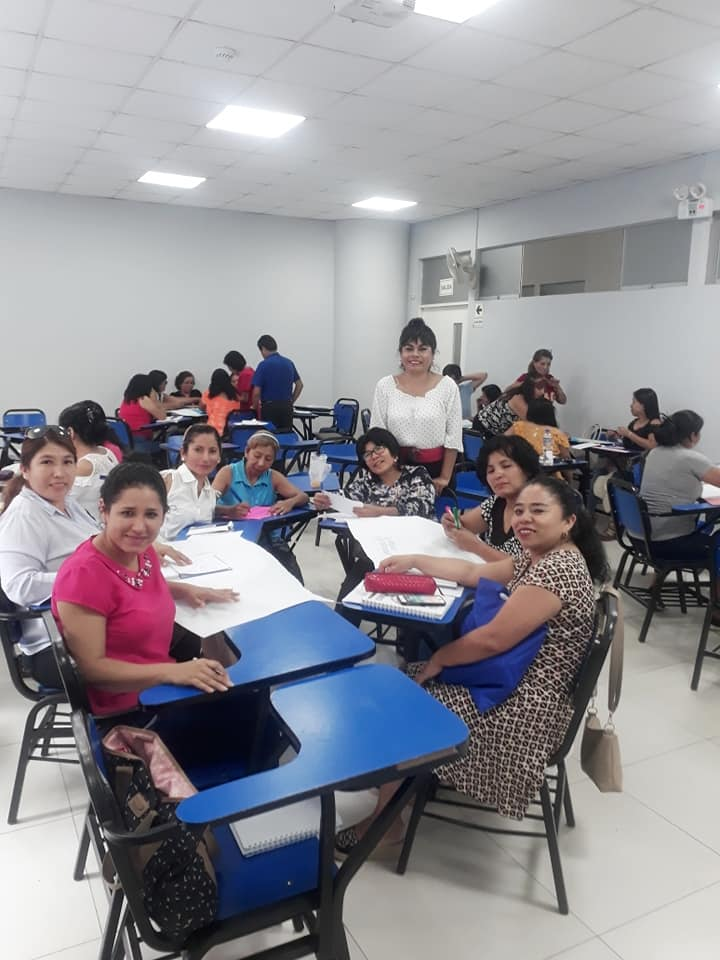
\includegraphics[width=300px]{../img/rosa.jpeg}
	\caption{Rosa Diaz Fonseca (rechtstaand) tijdens een bijscholing voor leerkrachten }
	\label{rosa}
\end{figure}


\section{Interview}

\textbf{Hoeveel leerlingen zitten er gemiddeld in de klassen van uw school?}

\textit{Rosa:} Er zitten gemiddeld ongeveer 33 leerlingen in elke klas. Op mijn school zijn er 8 klaslokalen. De volledige school telt ongeveer 265 leerlingen.

\textbf{Hebben de kinderen thuis toegang tot een computer?}

\textit{Rosa:} Peru telt verschillende maatschappelijke klassen. Er is een onderklasse, middenklasse en bovenklasse. De meeste kinderen op mijn school komen uit de onderklasse. Die kinderen komen uit arme gezinnen die geen computers ter beschikking hebben. Over het algemeen geldt er dat kinderen uit de midden- en bovenklasse thuis wel computers hebben.

\textbf{Heeft jouw school computers ter beschikking? Welke apparatuur is er? Zijn er problemen met deze apparatuur?}

\textit{Rosa:} De school heeft 32 computers, maar het zijn geen moderne computers. Het zijn kleine educatieve computers van het type XO95. Ze zijn wit en groen van kleur. De overheid besliste een aantal jaar geleden om veel geld in het XO project te pompen en veel computers aan te kopen. Ik denk dat ze betere computers met dat geld konden kopen. Het ging toen echt over gigantische bedragen. Op dit moment zijn de computers echt verouderd. Daardoor zijn ze onbruikbaar. De computerwereld verandert zo snel en onze overheid maakt geen geld vrij om die veranderingen op te volgen.

\textbf{Mogen de kinderen de XO computer meenemen naar huis?}

\textit{Rosa:} Neen, bij ons op school is dat niet de bedoeling. Ik weet dat dat op andere scholen in de binnenstad van Lima wel gebeurt.

\textbf{Als leerlingen informatica les krijgen, wat leren ze dan?}

\textit{Rosa:} De kinderen krijgen een basisopleiding schrijven en lezen. De computers worden gebruikt om dat te ondersteunen. Ze zouden toch gebruikt moeten worden als ondersteuning. In realiteit zijn de computers erg traag. Eigenlijk valt er weinig mee aan te vangen. Ze zijn erg verouderd.

\textbf{Heeft jouw school een ICT leerkracht?}

\textit{Rosa:} Niet alle scholen hebben informatica leerkrachten. Dit komt omdat de scholen te weinig budget krijgen van het Peruviaanse ministerie van onderwijs. Om die reden hebben wij dus geen leerkracht informatica. Een informatica leerkracht aanwerven is gewoonweg onbetaalbaar. Ik verwacht van mijn normale leerkrachten dat ze de taak van informatica leerkracht op zich nemen en de informaticakennis die ze hebben doorgeven aan de kinderen.

\textbf{In hoeverre kunnen uw gewone leerkrachten overweg met informatica?}

\textit{Rosa:} De leerkrachten geven hun informatica kennis die ze hebben door aan de leerlingen. Ik weet dat het beter zou zijn mocht er een informatica leerkracht zijn, maar die is er niet.

\textbf{Krijgen leerlingen huiswerk op de computer?}

\textit{Rosa:} Ja, de kinderen hebben huiswerk op computer maar maken dat niet thuis. Zoals ik al zei hebben er velen thuis geen computers, en dus gaan ze naar internetcafés. Daar kunnen ze een computer gebruiken om huiswerk op te maken. Echter, in een internetcafé wordt er geen toezicht gehouden op de kinderen. Daarom spelen ze daar vaak spelletjes op de computer en gebruiken ze niet al hun tijd om hun huiswerk te maken. De computers die ze ter beschikking hebben, hebben meestal geen veilig internet voor kinderen. De kinderen zouden per ongeluk op pornografische websites of andere kwaadaardige websites terecht kunnen komen. Daar maak ik me zorgen over.

\textbf{Hoe komt het dat Peru niet verder staat op vlak van informatica, wat liep er fout in het verleden?}

\textit{Rosa:} Eén van de grote problemen in het onderwijs van Peru is het nationale budget dat wordt gespendeerd aan de educatie van kinderen. Volgens mij beseffen ze vaak niet wat de kracht van onderwijs is. 

Daarnaast hebben ongeveer de helft van de scholen geen document dat aantoont dat de schoolgebouwen eigendom zijn van de staat. Er is een wet in Peru die stelt dat de overheid slechts kan investeren in de infrastucuur en gebouwen van de scholen als zij ook de eigendomsrechten heeft. De Peruviaanse overheid laat na dit administratief correct te notuleren, waardoor ze niet gedwongen kan worden te investeren.

Er is veel corruptie. Niet elke school wordt gelijk bedeeld. De scholen die ondersteund worden door de overheid zijn vaak scholen in de hoofdstad waar veel kinderen uit de middenklasse naar toe gaan. Als scholen niet door de staat gefinancierd worden, gebeurt het dat ouders zelf collectes doen om de school te steunen. De meeste computers op staatsscholen worden aangekocht met steun van ouders die actie ondernamen. 

\textbf{Je gaf ook opleidingen aan leerkrachten. Was er bijscholing voor informatica?}

\textit{Rosa:} De leerkrachten moeten zichzelf bijscholen op vlak van informatica. We gebruikten tijdens deze lessen wel computers om filmpjes te kijken of om dia-voorstellingen te bekijken, maar echt bijscholing specifiek voor ICT was er niet. Als een leerkracht bijscholing informatica wil zal hij daar zelf voor moeten betalen.

\textbf{Heb je op dit moment als directrice zelf geen extra mogelijkheden om de informatica binnen jouw school te verbeteren?}

\textit{Rosa:} We hebben geprobeerd om een programma op te zetten om de informatica op onze school te verbeteren. Dat lukte niet omdat scholen in buitenwijken van de hoofdstad vaak een tekort aan de meest elementaire basis hebben. Er is geen stroom, stromend water of riolering in deze wijken! Niet alleen scholen hebben te maken met dit probleem, maar ook andere instanties zoals medische posten, die men wil opbouwen in een buitenwijk hebben hier vaak mee te kampen. Mijn school is één van de vele scholen die dit probleem heeft. De overheid zou dit eerst moeten oplossen vooraleer we zelf kunnen denken aan nieuwe computers op school. De huidige XO laptops werken op zonne-energie. 

\textbf{Wat zouden mogelijke oplossingen kunnen zijn voor deze problemen?}

\textit{Rosa:} Ik denk dat de lokale overheden beter zouden moeten functioneren. Als zij zouden instaan voor de basis infrastructuur zouden daar veel initiatieven mee geholpen zijn. Ze zouden water, elektriciteit en rioleringen moeten aanleggen. Op dit moment bundelen we de krachten met een aantal lokale instituten om dit toch zelf te kunnen verwezenlijken, maar dat is niet eenvoudig. 

Donaties zouden ook kunnen helpen. Er kunnen activiteiten georganiseerd worden om geld te verdienen. Ik denk dan aan tombola's of eetfestijnen. Met dat geld zouden er dan computers aangekocht kunnen worden. NGO's zouden ons ook kunnen helpen. Laatst nog stond ik in contact met een NGO die ons wou helpen met het opwekken van elektriciteit van de zon om zo toch elektriciteit te hebben op onze school.

\subsection{Factcheck}
%olpc XO95
Ook op de school van Mevr. Diaz Fonseca worden de OLPC XO computers gebruikt. Volgens Rosa pompte Peru veel geld in OLPC. Dat blijkt ook uit de stand van zaken in sectie \ref{olpc-in-peru}, waar beschreven staat dat in Peru het grootste OLPC programma uitgerold werd. Mevr. Diaz Fonseca vertelt ook dat er op haar schol XO95 laptops gebruikt worden. Dat klopt niet. Het type XO95 bestaat niet. Alleen de types XO-1, XO-1.5, XO-1.75, XO-2, XO-3 en XO-4 Touch werden ontworpen. \autocite{OLPC2016}. Nochtans komt haar beschrijving op vlak van de kleuren duidelijk overeen. Ze vergist zich waarschijnlijk in een van deze versies.

Mevr. Diaz Fonseca spreekt ook over een probleem met eigendomsaktes van scholen. In 2004 was 75\% van de scholen in Peru gevestigd in gebouwen die geen wettelijke fysieke sanitaire voorzieningen heeft. Dat komt omdat ze geen eigendomsaktes hebben. Volgens het openbaar register bestaan ze niet. Dit percentage komt overeen met meer dan 31.000 scholen over heel Peru. Zoals Rosa uitlegt zijn de eigendomsaktes belangrijk om te kunnen investeren in scholen. Als er aanpassingen aan de infrastructuur van een pand of de accommodatie moeten gebeuren, met steun via overheidsgeld, is een eigendomsakte nodig die duidelijk maakt dat de grond geen verplichtingen jegens derden heeft en vrij is van pandrechten. Als dit niet het geval is maakt men geen kans op subsidies, en kan men de scholen niet voorzien van sanitaire voorzieningen.

Het echte probleem is dat de staat niet over de middelen beschikt om deze onderwijsfaciliteiten onmiddellijk te verbeteren. Daarom starten ze weinig procedures op om de eigendomsaktes in orde te brengen. De procedure om eigendomsaktes op te stellen kost trouwens ongeveer 1000 sol (+/- 270 euro) per school. Dat betekent dat er ongeveer 31 miljoen sol (+/-8,4 miljoen euro) nodig is om de eigendomsaktes van de overige 75\% van de scholen in orde te brengen. Volgens de overheid gaat dit om te veel geld dat ze beter op andere manieren kan investeren. \autocite{larepublica2004}

% Voeg hier je eigen hoofdstukken toe die de ``corpus'' van je bachelorproef
% vormen. De structuur en titels hangen af van je eigen onderzoek. Je kan bv.
% elke fase in je onderzoek in een apart hoofdstuk bespreken.

%\input{...}
%\input{...}
%...



\chapter{Conclusie}
\label{ch:conclusie}

% onderzoeksvra(a)g(en). Wat was jouw bijdrage aan het onderzoeksdomein en
% hoe biedt dit meerwaarde aan het vakgebied/doelgroep? 
% Reflecteer kritisch over het resultaat. In Engelse teksten wordt deze sectie
% ``Discussion'' genoemd. Had je deze uitkomst verwacht? Zijn er zaken die nog
% niet duidelijk zijn?
% Heeft het onderzoek geleid tot nieuwe vragen die uitnodigen tot verder 
%onderzoek?

\section{Inleiding}
Uit de interviews kwamen een aantal duidelijk gelijklopende, maar ook een aantal verschillende meningen naar voor. De drie interviews werden afgenomen van drie personen uit drie verschillende regio's. Hun ervaring, achtergrond, leeftijd, type  scholen of projecten waren uiteraard verschillend, maar geven toch een vrij uniform beeld weer van de situatie in Peru. Via deze informatie zal er in dit hoofdstuk een antwoord geformuleerd worden op volgende onderzoeksvragen:

$Onderzoeksvraag$ 1: Wat is de huidige stand van zaken op vlak van ICT binnen het onderwijs in Peru, en hoe is het land hiertoe gekomen?

$Onderzoeksvraag$ 2: Hoe kunnen deze knelpunten weggewerkt worden in de toekomst, en hoe is het land hiertoe gekomen?

\section{Wat is de huidige stand van zaken op vlak van ICT binnen het onderwijs in Peru?}
Uit de interviews kwamen een aantal duidelijke knelpunten naar boven:

% verschillen tussen de interviews bespreken, en afleiden naar grote varieteit


\subsection{Slechte basis fundamenten}
Uit de interviews bleek meerdere malen dat de basis fundamenten (water, elektriciteit,... ) in veel gebieden in Peru niet beschikbaar is. Dat kan komen door de typische geografie van het land maar ook door het wanbeleid van de regering. Als men vooruit wil gaan op het vlak van informatica zou de overheid er voor moeten zorgen dat minstens de basisbehoeften in orde zijn. Stromend water, rioleringen en elektriciteit zouden overal een evidentie moeten zijn. Echter is dat vandaag niet overal het geval.

\subsection{Te weinig werkmiddelen vanuit het ministerie van onderwijs}
Voor de voorbije regeringen was onderwijs duidelijk geen prioriteit. Het is belangrijk dat een overheid begrijpt wat onderwijs kan betekenen voor de toekomst van een land. Doordat onderwijs geen prioriteit was in het verleden werden er te weinig werkmiddelen en budgetten vrijgemaakt.

\subsection{Huidige informatica infrastructuur verouderd}
De Peruviaanse regering sprong in 2007 op de kar toen de XO laptops geproduceerd en verdeeld werden. Dit was een goede zaak voor het land, omdat er veel leerlingen voor het eerst in aanraking kwamen met informatica. Ondanks de kwalen functioneerden de XO laptops goed toen ze werden aangekocht. Op dit moment zijn de laptops echter verouderd. Ze zijn daardoor compleet onbruikbaar geworden.

\subsection{Te kort aan informatica-bijscholing voor leerkrachten}
Vaak zijn er geen opgeleide informatica leerkrachten op scholen. Daarom zou het goed zijn om het niveau van informaticakennis bij elke leerkracht op te krikken, zodat ze met hun kennis minstens een volwaardige les informatica kunnen 	aanbieden aan de leerlingen. Als leerkrachten toch bijscholing informatica willen volgen, moeten ze dat vandaag op eigen houtje doen en er soms zelfs zélf voor betalen. Jonge leerkrachten hebben vaak meer voeling met ICT dan leerkrachten met een lange staat van dienst. Net voor hen zou het erg zinvol kunnen zijn om deze nieuwe technologieën te kunnen hanteren. 

\subsection{Te kort aan informatica leerkrachten}
Niet elke school in Peru heeft een leerkracht informatica. Dat komt omdat er in een aantal regio's geen opleiding is tot informatica leerkracht. Vaak moeten er dus andere, onopgeleide leerkrachten inspringen of moet er gekeken worden naar ICT-specialisten om informatica les te geven. In het geval er gekozen wordt voor andere leerkrachten hebben die meestal geen bijscholing informatica gevolgd. Als er naar een specialist gekeken wordt zijn die vaak te duur voor de scholen. 

\subsection{Te veel armoede in het algemeen}
Er is te veel armoede in sommige regio's in Peru. Gezinnen hebben daar niet genoeg financiële middelen om rond te komen. Als dit het geval is zijn ze al zeker niet in staat om een computer aan te kopen voor het gezin. Daardoor kunnen de kinderen thuis hun huiswerk niet maken en gaan ze vaak naar internetcafés. Daar is er geen toezicht en kan de aandacht sneller afglijden naar andere zaken zoals videospelletjes of kunnen ze, in het slechtste geval, op kwaadaardige websites terecht komen.

\section{Hoe kunnen deze knelpunten weggewerkt worden in de toekomst?}

\subsection{Peruviaanse overheid}
%basisfundering, extra steun opleidingen aanbieden, leerkrachten bijles geven
De overheid zou in de toekomst werk moeten maken van investeringen in het onderwijs. Ze zouden minsten de basis fundamenten voor stromend water, rioleringen en elektriciteit moeten voorzien voor scholen, zodat projecten die vanuit de school worden georganiseerd kunnen doorgaan. Er zou ook meer budget moeten voorzien worden voor het ministerie van onderwijs. Als dat kan zou een nieuwe grootschalige aankoop van computers voor in scholen, zoals ze dat deden voor de XO-laptops, heel erg nuttig zijn voor de leerlingen. 

\subsection{Ministerie van onderwijs}
Het ministerie van onderwijs zou ervoor moeten zorgen dat men overal in Peru een opleiding tot leerkracht ICT kan volgen. Daarnaast zou elke school moeten voorzien in een informatica leerkracht die de infrastructuur kan beheren en les kan geven aan de leerlingen. Ook het basis informatica niveau van andere leerkrachten zou omhoog gekrikt moeten worden. Dat zou perfect gaan via bijscholing op de manier zoals het nu al gebeurt. Indien er meer budget kan voorzien worden vanuit de overheid zouden deze doelstellingen kunnen behaald worden.

\subsection{Steun via NGO's}
Steun via NGO's kan een verschil maken voor informatica in onderwijs. Grote bedrijven kunnen helpen door kortingen te geven aan scholen en andere organisaties zonder winstoogmerk. Zo heeft Microsoft bijvoorbeeld op dit moment een programma, genaamd "Microsoft for Education", waarmee ze informatica in het onderwijs willen stimuleren. Door het verlagen van het prijskaartje kan dit soort initiatieven de aankoop van IT materiaal faciliteren.

%Dit soort initiatieven kunnen de vaak te hoge drempel, die zich meestal uit in het veel te hoge prijskaartje, weg halen voor scholen. 

Daarnaast zouden kleinschaligere initiatieven ook hun nut kunnen hebben. Zo zouden er bijvoorbeeld verouderde computers kunnen ingezameld worden. Meestal zijn verouderde computers te oud, omdat de nieuwe software meer capaciteit nodig heeft. Daarom zou er een licht besturingssysteem kunnen ontworpen worden, speciaal gericht op kinderen en educatie. Die software kan dan geïnstalleerd worden op oude computers, die dan verdeeld zouden kunnen worden onder scholen. Zo zouden een hele hoop oude computers gerecycleerd kunnen worden, en toch nuttig zijn in het onderwijs.

\section{Toekomstig onderzoek binnen dit domein}

Een aantal toekomstige onderzoeken binnen dit domein zouden kunnen zijn: 
\begin{itemize}
	\item Wat was de impact van het covid-19 virus op informatica in het onderwijs in Peru?
	\item In hoeverre verbeteren schoolresultaten als er gebruik gemaakt wordt van informatica tijdens het leerproces?
\end{itemize}



%%=============================================================================
%% Bijlagen
%%=============================================================================

\appendix
\renewcommand{\chaptername}{Appendix}

%%---------- Onderzoeksvoorstel -----------------------------------------------

\chapter{Onderzoeksvoorstel}

Het onderwerp van deze bachelorproef is gebaseerd op een onderzoeksvoorstel dat vooraf werd beoordeeld door de promotor. Dat voorstel is opgenomen in deze bijlage.

% Verwijzing naar het bestand met de inhoud van het onderzoeksvoorstel
%---------- Inleiding ---------------------------------------------------------

\section{Introductie} % The \section*{} command stops section numbering
\label{sec:introductie}

In de wereld heerst nog steeds  verdeeldheid ondanks we er op vele vlakken op vooruit gaan. In de meeste landen van  Europa en Noord-Amerika stellen de burgers het goed. Er is genoeg voedsel, toegang tot goede gezondheidszorg, een uitgebouwd onderwijssysteem, en ga zo maar door. Dat is niet overal het geval. Veel landen hebben te kampen met snelle bevolkingsgroei, hoge sterftecijfers en een grote kloof tussen arm en rijk. Veelal hebben deze landen een ontwikkelingsachterstand. 
%https://www.un.org/development/desa/dpad/wp-content/uploads/sites/45/WESP2019_BOOK-web.pdf

Er werd al veel onderzoek gedaan naar hoe ICT invloed kan hebben op de ontwikkeling van een land. Dit onderzoek zal zich specificeren op ICT in het onderwijs in Peru. Het heeft als doel de invloed van ICT op het niveau van het onderwijs in Peru te analyseren, en te onderzoeken hoe dit kan verbeterd worden. 

%---------- Stand van zaken hehe ---------------------------------------------------

\section{Stand van zaken}
\label{sec:state-of-the-art}
Ontwikkelingslanden hebben economische, technologische, wetenschappelijke en medische achterstanden tegenover ontwikkelde landen. De Verenigde naties deelt alle landen van de wereld op in 3 tabellen. Daaruit blijkt dat er 43 ontwikkelde landen, 17 landen de overgang aan het maken zijn tussen ontwikkeld en onderontwikkeld, en 127 onderontwikkelde landen zijn. \autocite{unitednations2019} Peru behoort bij de laatste groep van de onderontwikkelde landen. 

Sinds de jaren '90 heeft informatie communicatie technologie (ICT) veel invloed op onze samenlevingen. Op vele vlakken evolueren we heel snel door middel van ICT. Door deze nieuwe trend veranderde ons leven, en kunnen we zaken  effici\"enter doen. In Peru heeft op dit moment 53\% van de bevolking toegang tot het internet, tegenover 89\% in Belgi\"e. \autocite{itu2018} Ook op vlak van onderwijs kan er ge\"evolueerd worden, om zo de kwaliteit van het onderwijs te verbeteren.

In 2001 werd het Huascaran Project opgestart in Peru. Het doel van het project was om landelijke netwerken te ontwikkelen, implementeren en evalueren voor openbare scholen en het uitrusten van deze scholen met een server en toegang tot internet. Om op die manier de kwaliteit van het onderwijs te verbeteren. Er werden ongeveer 15.000 computers verspreid over scholen in het hele lang en 55.000 leraren werden opgeleid. Echter, het project werd nooit ge\"evalueerd, en eindigde in 2007.  \autocite{salas-pilco2014}

In 2007 startte het wereldwijde 'One Laptop Per Child' gen\"introduceerd in Peru. Dat was een project met als doel, elk kind op school te voorzien van een laptop, om zo het onderwijs naar een hoger niveau te tillen. Nicholas Negroponte, de vader van het project, was gericht op het beëindigen van armoede door middel van computers. Hij ontwierp een apparaat om de Derde Wereld te helpen. Dat project faalde, door vele projectmatige fouten. \autocite{Wooster2018} Over of het project nu echt de kinderen slimmer maakte, is er onenigheid: een studie \autocite{Severin2012} van de Inter-Amerikaanse Ontwikkelingsbank wees uit dat Peruaanse kinderen met laptops zes maanden voorsprong hadden op hun leeftijdsgenoten op vlak van logisch redeneren en hun verbaal vermogen, maar het onderzoek kon  geen verbeteringen vinden op gebieden als wiskunde, taal of leesgewoonten. \autocite{Murhpy2012}
 

%---------- Methodologie ------------------------------------------------------
\section{Methodologie}
\label{sec:methodologie}
De desk research zal gebeuren door de literatuur die al over ICT en educatie in Peru werd geschreven te analysen. Het verdere field research zal plaatsvinden door ter plaatse te gaan, en via vragenlijsten zal gekeken worden wat de bevindingen van de Peruvianen zelf zijn.
 
 %beschrijf je hoe je van plan bent het onderzoek te voeren. Welke onderzoekstechniek ga je toepassen om elk van je onderzoeksvragen te beantwoorden? Gebruik je hiervoor experimenten, vragenlijsten, simulaties? Je beschrijft ook al welke tools je denkt hiervoor te gebruiken of te ontwikkelen.

%---------- Verwachte resultaten ----------------------------------------------
\section{Verwachte resultaten}
\label{sec:verwachte_resultaten}
Er wordt verwacht dat er in de publieke scholen in Peru nog  onvoldoende aandacht is voor ICT. Er zou dus weinig of geen gebruik worden gemaakt van ICT tijdens het onderwijzen. Veelal wordt er gebruik gemaakt van traditionele methoden.
%Hier beschrijf je welke resultaten je verwacht. Als je metingen en simulaties uitvoert, kan je hier al mock-ups maken van de grafieken samen met de verwachte conclusies. Benoem zeker al je assen en de stukken van de grafiek die je gaat gebruiken. Dit zorgt ervoor dat je concreet weet hoe je je data gaat moeten structureren.

%---------- Verwachte conclusies ----------------------------------------------
\section{Verwachte conclusies}
\label{sec:verwachte_conclusies}
Vermoedelijk zou dit kunnen komen omdat Peru een onderontwikkeld land is. Hierdoor heeft het land geen budget om te investeren in ICT.
%Hier beschrijf je wat je verwacht uit je onderzoek, met de motivatie waarom. Het is \textbf{niet} erg indien uit je onderzoek andere resultaten en conclusies vloeien dan dat je hier beschrijft: het is dan juist interessant om te onderzoeken waarom jouw hypothesen niet overeenkomen met de resultaten.



%%---------- Andere bijlagen --------------------------------------------------
%: Voeg hier eventuele andere bijlagen toe
%\input{...}

%%---------- Referentielijst --------------------------------------------------

\printbibliography[heading=bibintoc]

\end{document}
